\documentclass[a4paper,11pt,titlepage]{bxjsarticle}
\usepackage[dvipdfmx]{graphicx}
\usepackage{listings}
\usepackage{amsmath}
\usepackage{fancybox,ascmac}
\usepackage{url}
\title{画像処理 課題3}
\author{175751C 宮城孝明}
\date{\today}
\begin{document}
\maketitle
\tableofcontents
\clearpage
\section{トーンカーブ変換}
\subsection{ソースコード}
\lstinputlisting[language=python, numbers=left, breaklines=true, basicstyle=\ttfamily\footnotesize,
  frame=single, caption=トーンカーブ, label=sample]{task1.py}
  
\subsection{実行結果}
\begin{figure}[htbp]
  \begin{center}
    \begin{tabular}{c}

      % 1
      \begin{minipage}{0.33\hsize}
        \begin{center}
          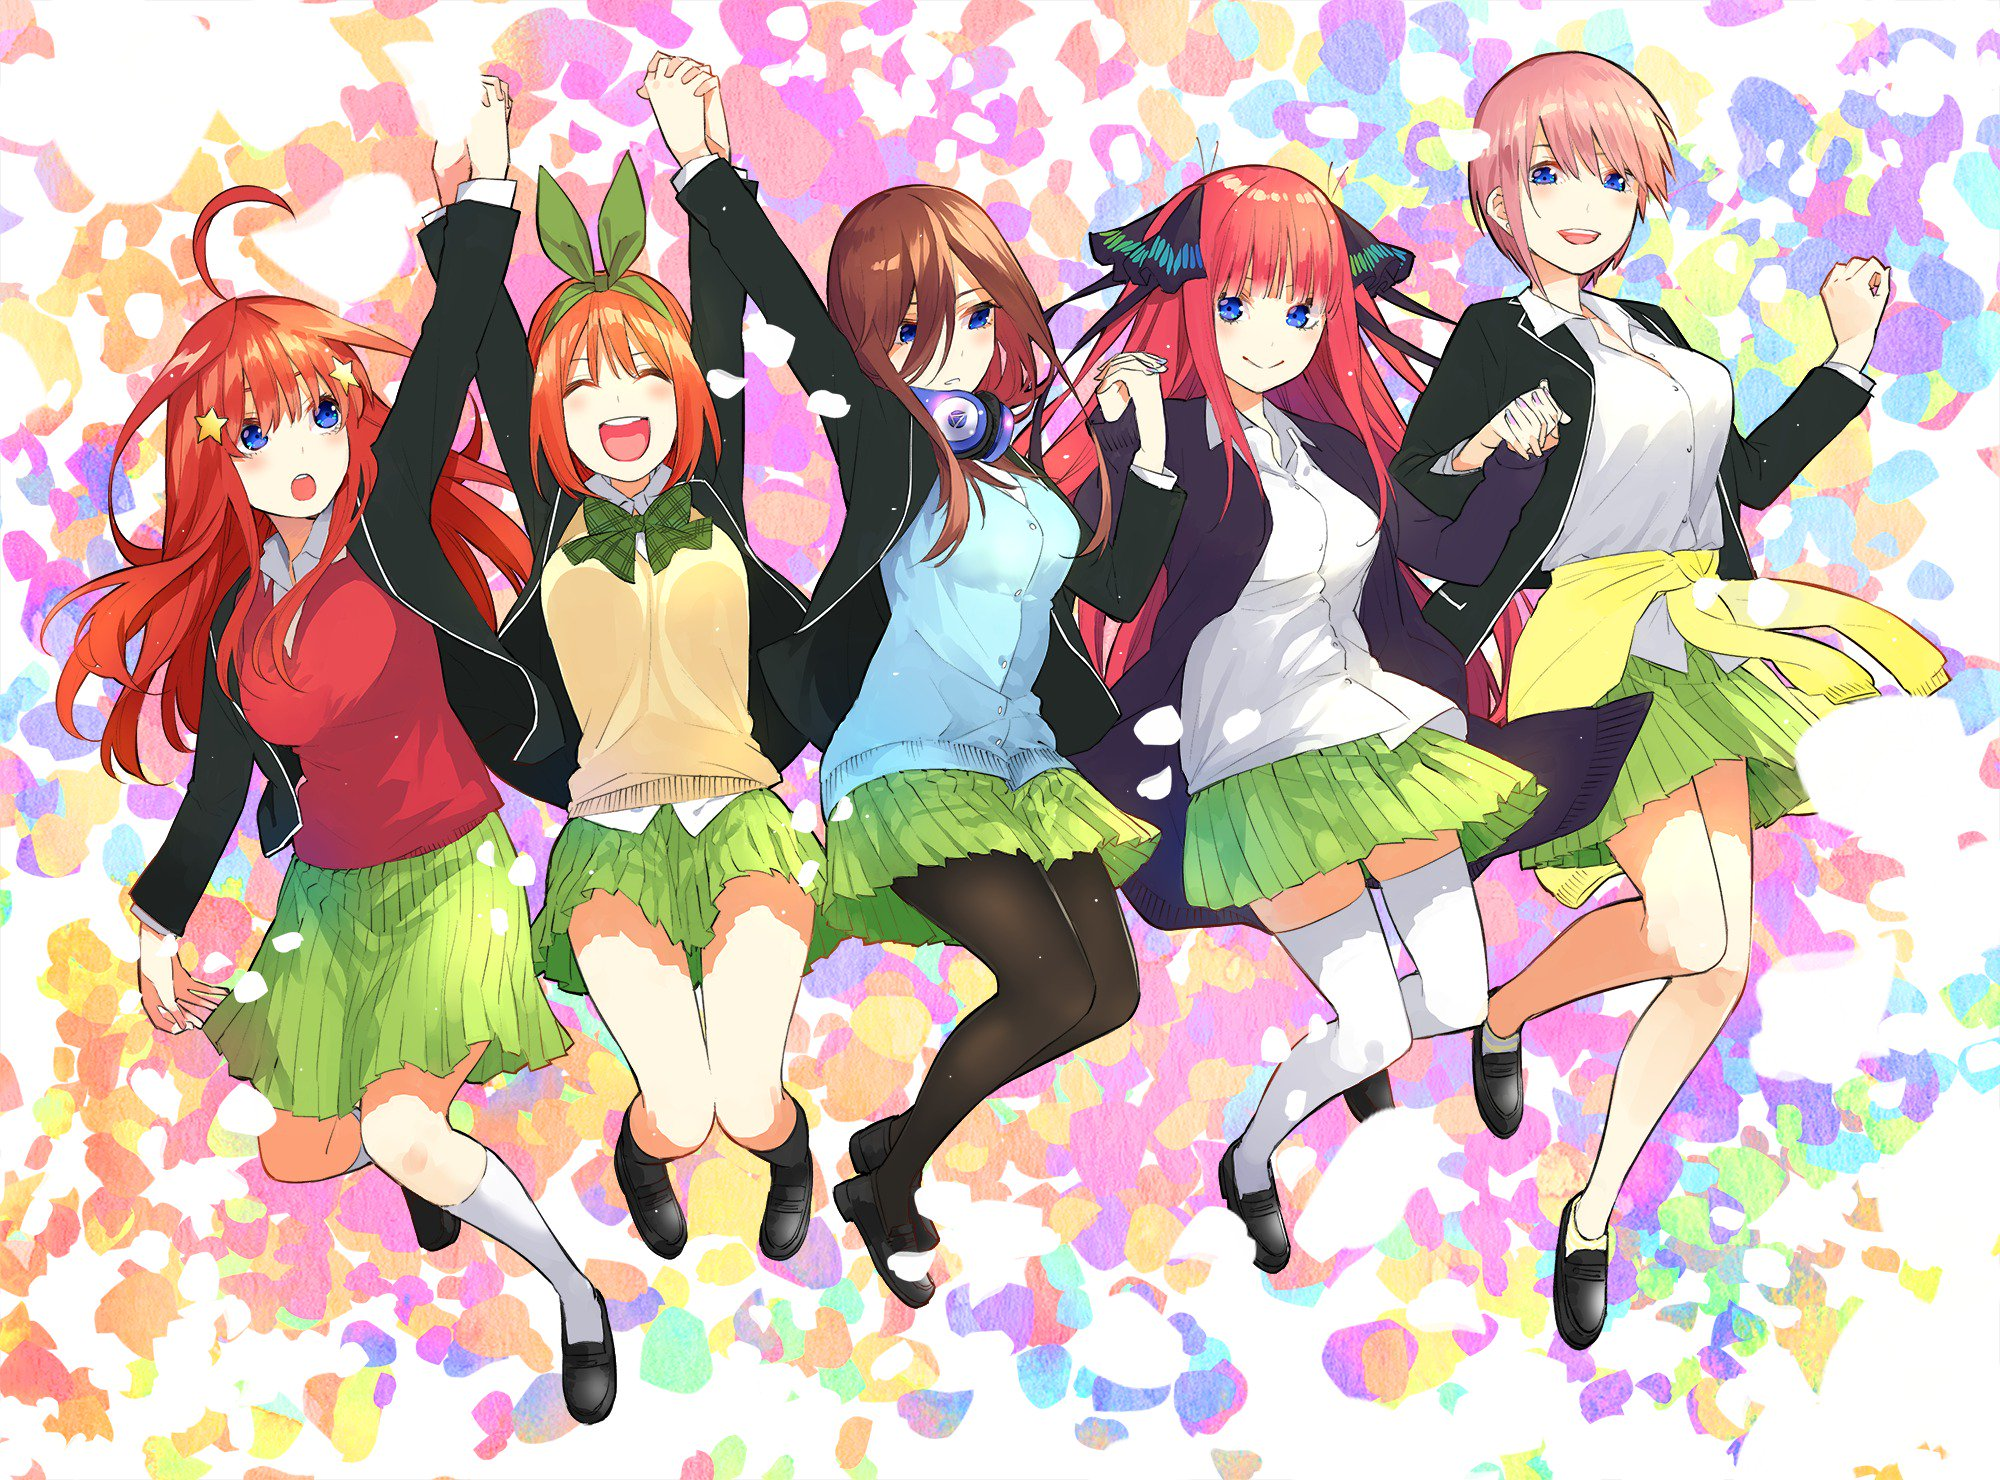
\includegraphics[clip, width=4.5cm]{./sample.jpg}
          \hspace{1.6cm} [1]通常画像
        \end{center}
      \end{minipage}

      % 2
      \begin{minipage}{0.33\hsize}
        \begin{center}
          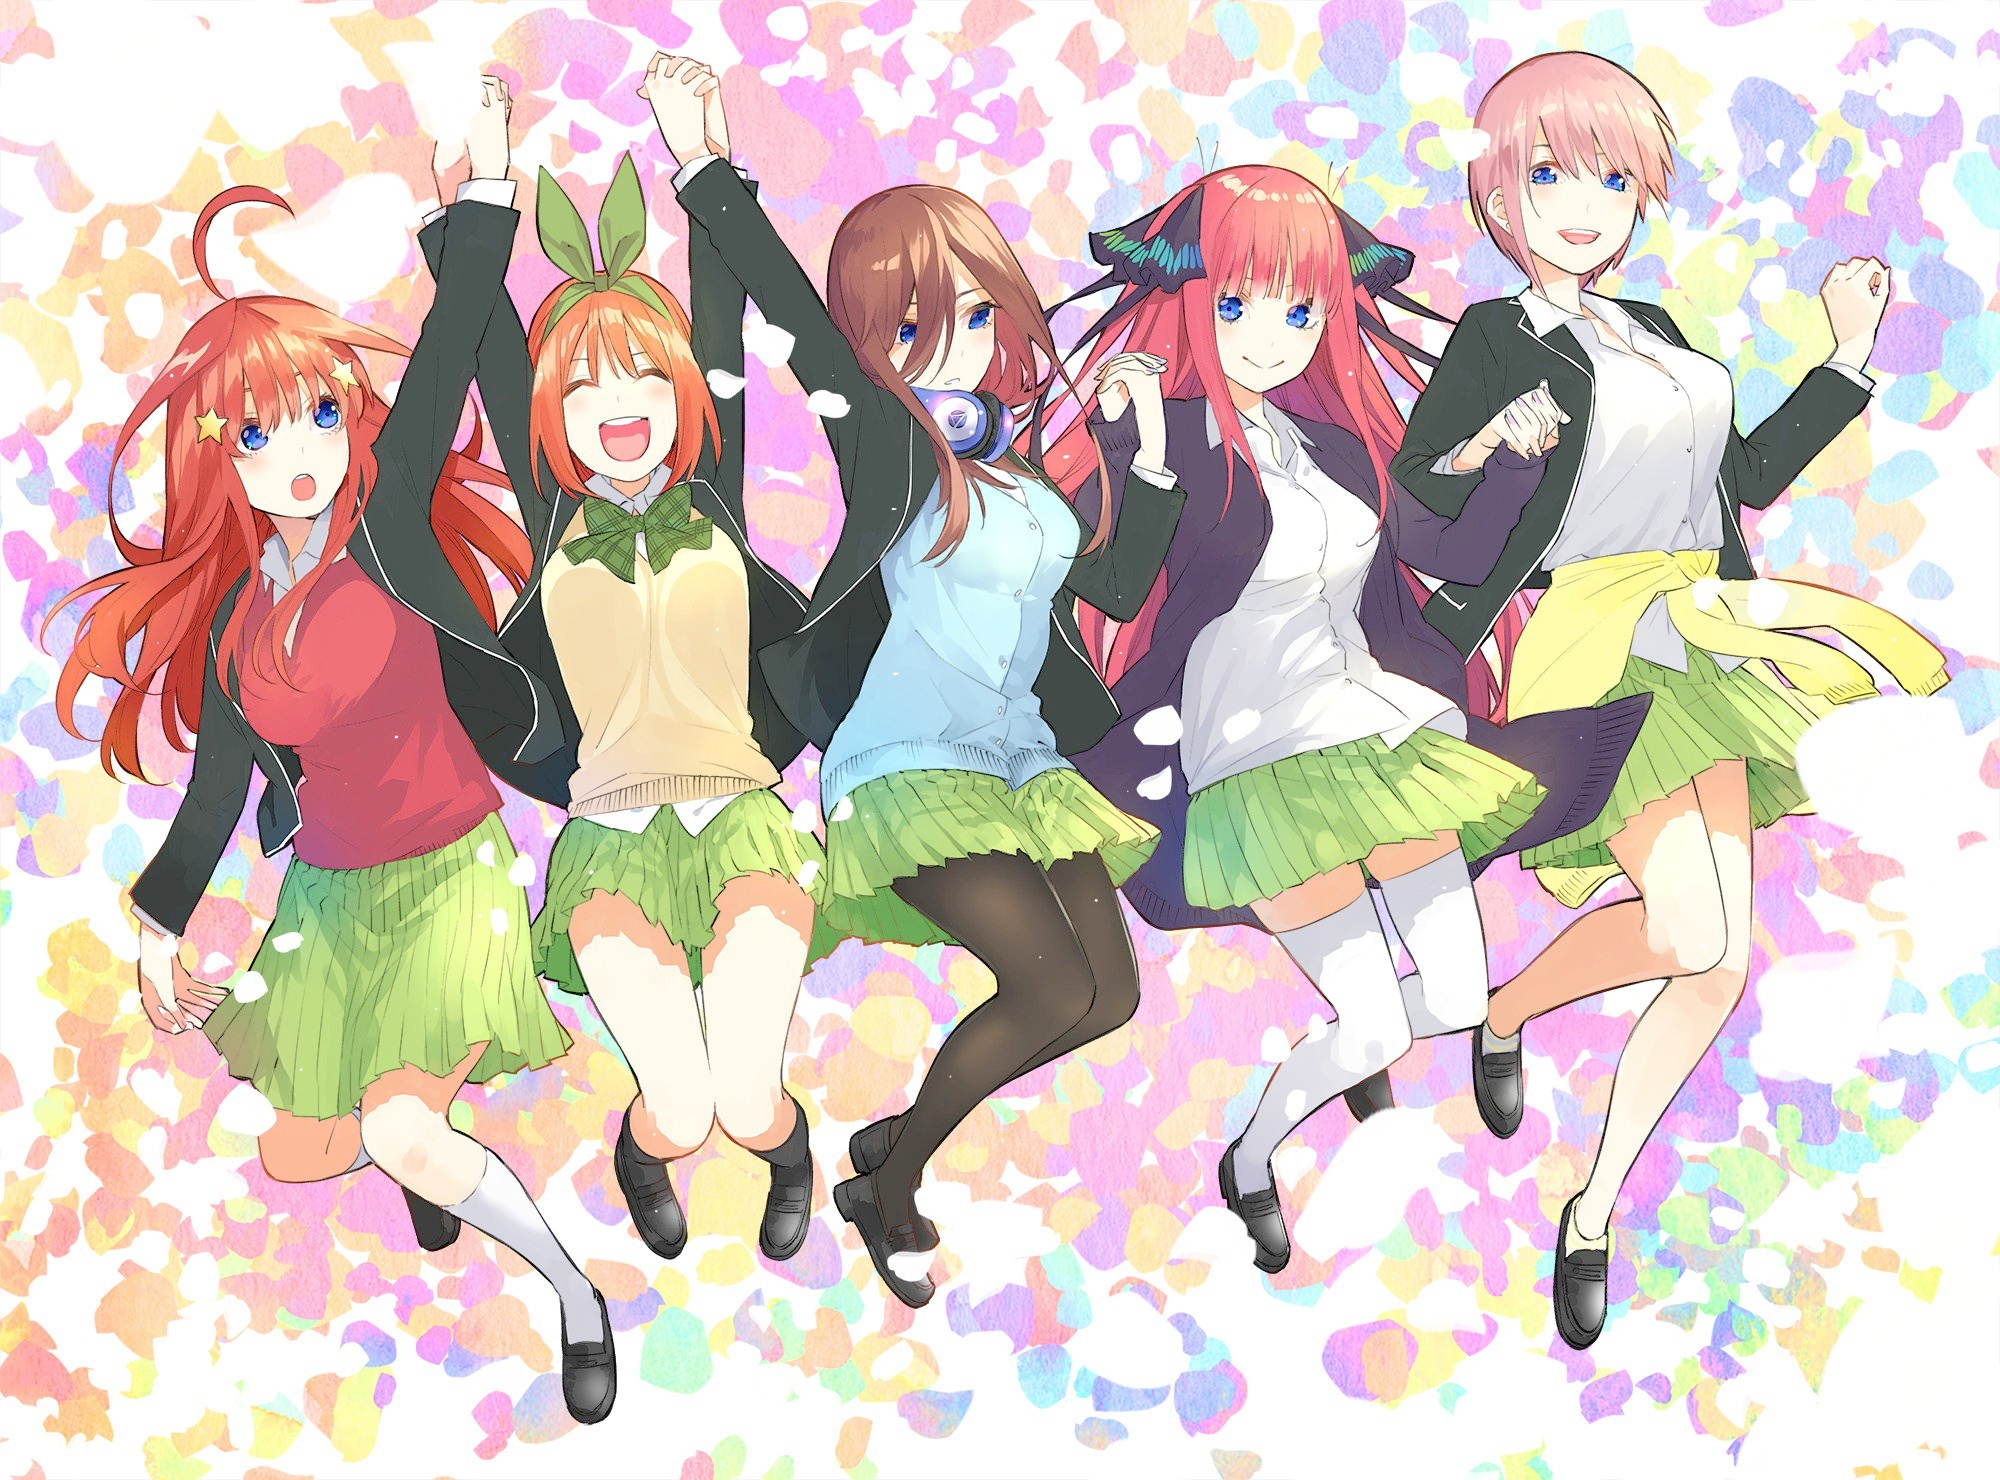
\includegraphics[clip, width=4.5cm]{./img_dst1.jpg}
          \hspace{1.6cm} [2]ganm=1.5
        \end{center}
      \end{minipage}

      % 3
      \begin{minipage}{0.33\hsize}
        \begin{center}
          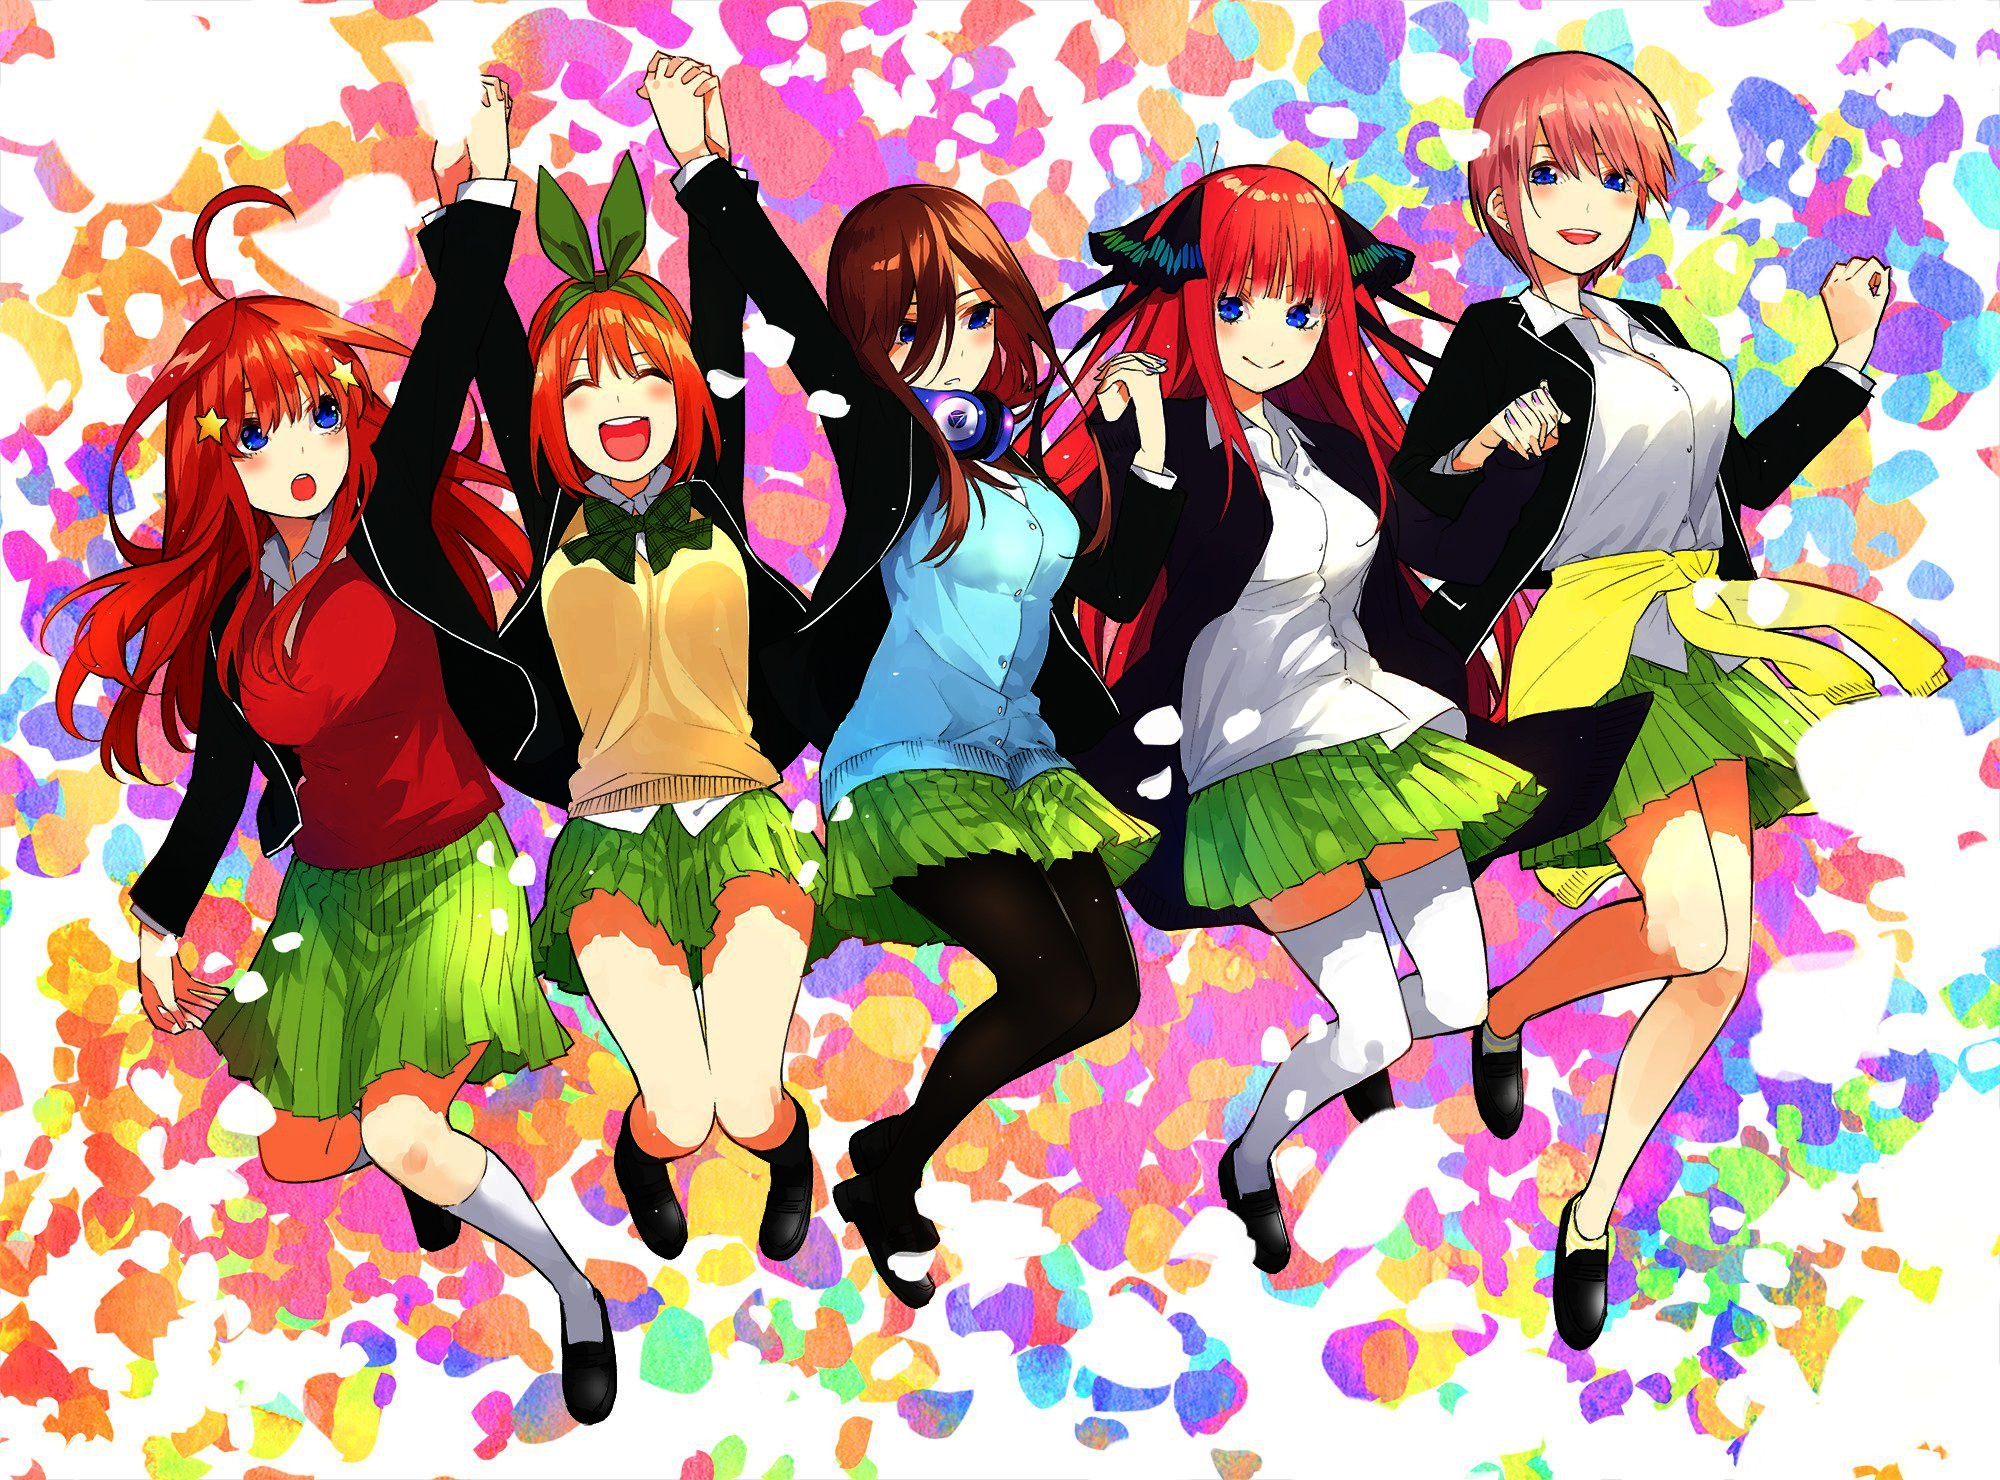
\includegraphics[clip, width=4.5cm]{./img_dst2.jpg}
          \hspace{1.6cm} [3]ganm=0.5
        \end{center}
      \end{minipage}

    \end{tabular}
    \caption{トーンカーブ}
    \label{fig:lena}
  \end{center}
\end{figure}

\section{アルファブレンディング}
\subsection{ソースコード}
\lstinputlisting[language=python, numbers=left, breaklines=true, basicstyle=\ttfamily\footnotesize,
  frame=single, caption=アルファブレンディング, label=sample]{abopencv.py}
\subsection{実行結果}
\begin{figure}[htbp]
  \begin{center}
    \begin{tabular}{c}

      % 1
      \begin{minipage}{0.33\hsize}
        \begin{center}
          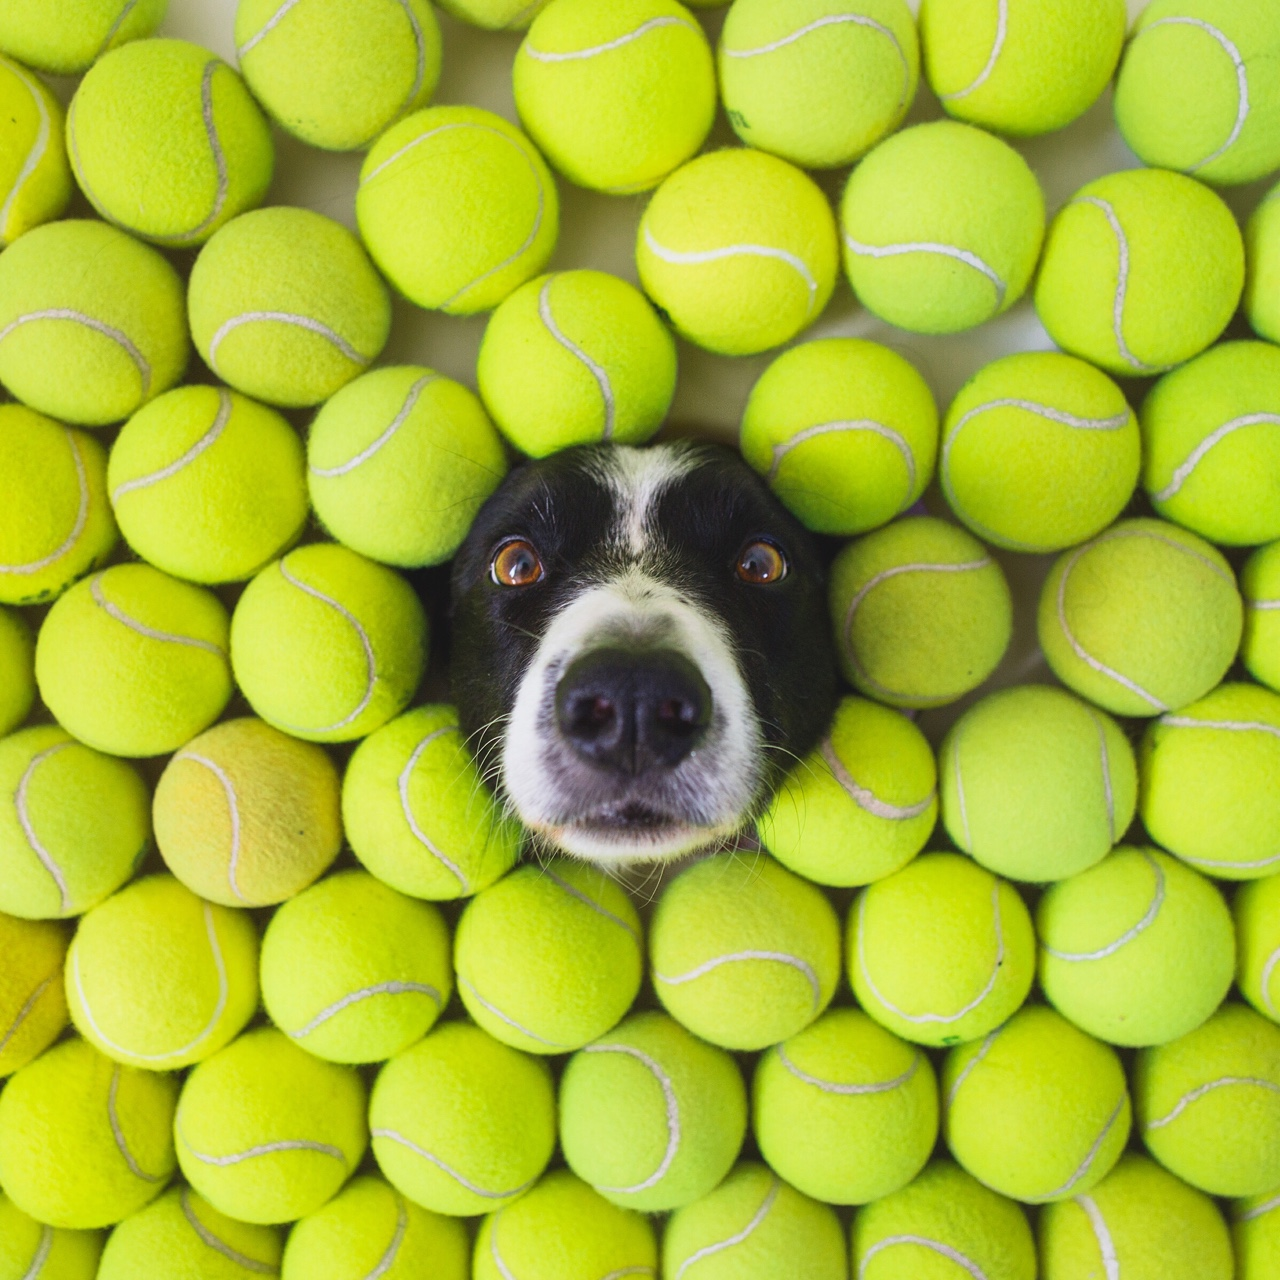
\includegraphics[clip, width=4.5cm]{./sample3.jpg}
          \hspace{1.6cm} [1]通常画像
        \end{center}
      \end{minipage}

      % 2
      \begin{minipage}{0.33\hsize}
        \begin{center}
          
\includegraphics[clip, width=4.5cm]{./sample4.jpg}
          \hspace{1.6cm} [2]通常画像
        \end{center}
      \end{minipage}

      % 3
      \begin{minipage}{0.33\hsize}
        \begin{center}
          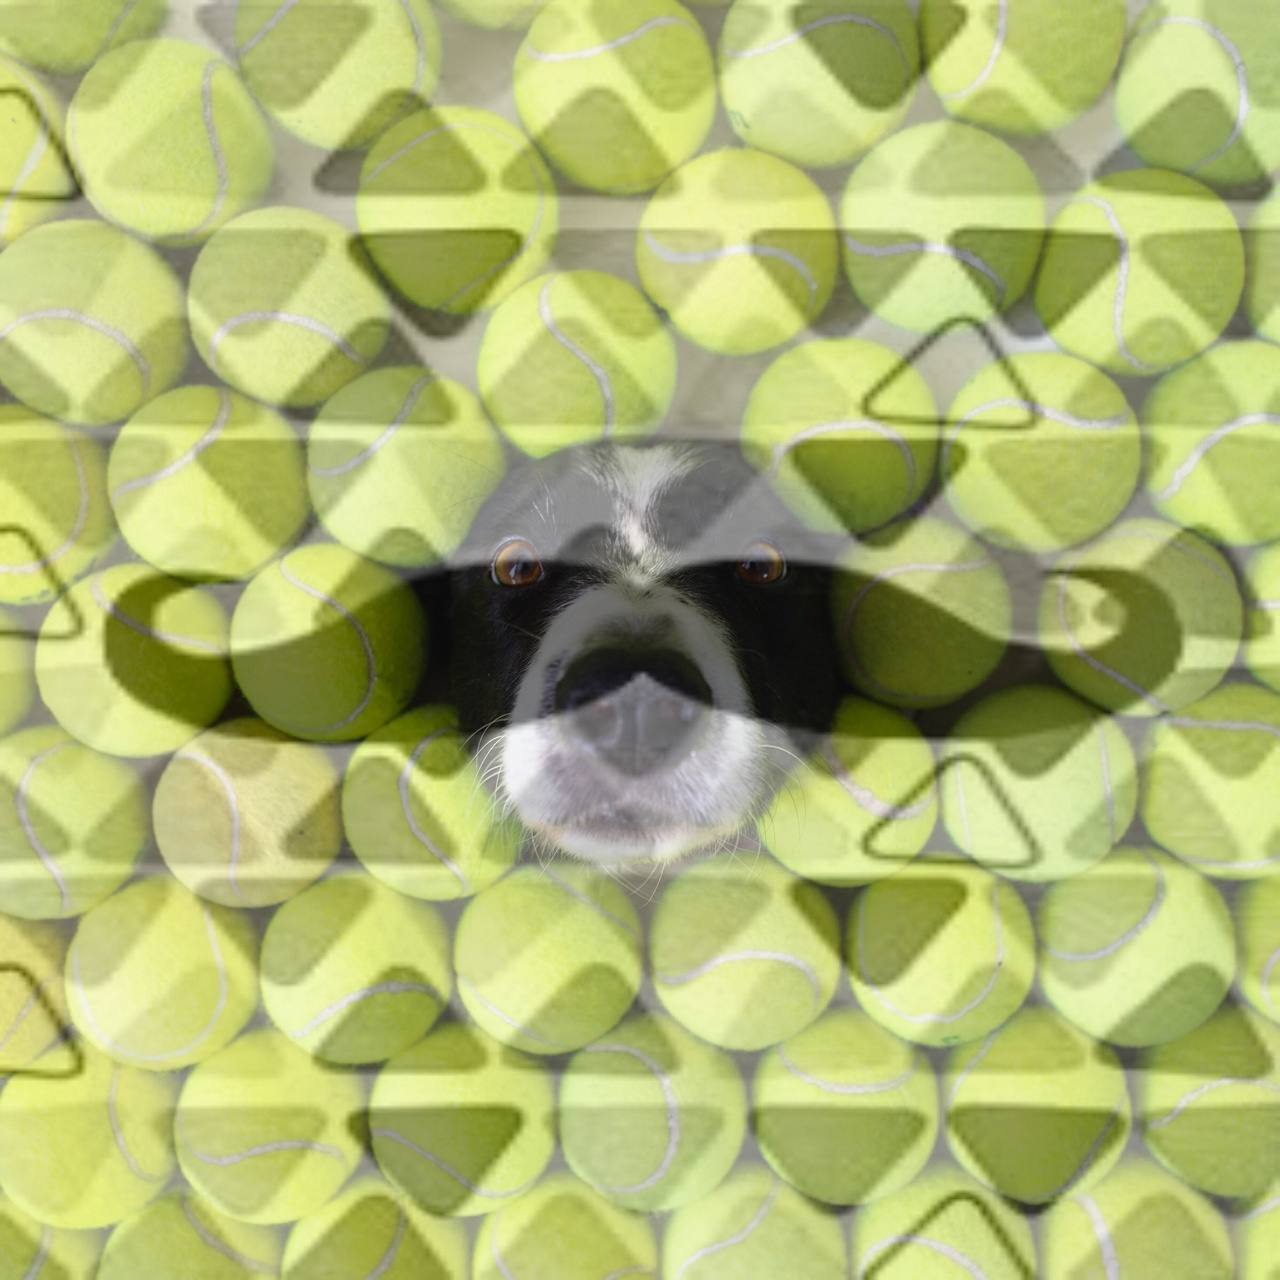
\includegraphics[clip, width=4.5cm]{./abdst.jpg}
          \hspace{1.6cm} [3]アルファブレンディング
        \end{center}
      \end{minipage}

    \end{tabular}
    \caption{アルファブレンディング}
    \label{fig:lena}
  \end{center}
\end{figure}

\section{左右反転}
\subsection{ソースコード}
\lstinputlisting[language=python, numbers=left, breaklines=true, basicstyle=\ttfamily\footnotesize,
  frame=single, caption=上下左右反転, label=sample]{Inversion.py}
\subsection{実行結果}
\begin{figure}[htbp]
  \begin{center}
    \begin{tabular}{c}
      % 1
      \begin{minipage}{0.33\hsize}
        \begin{center}
          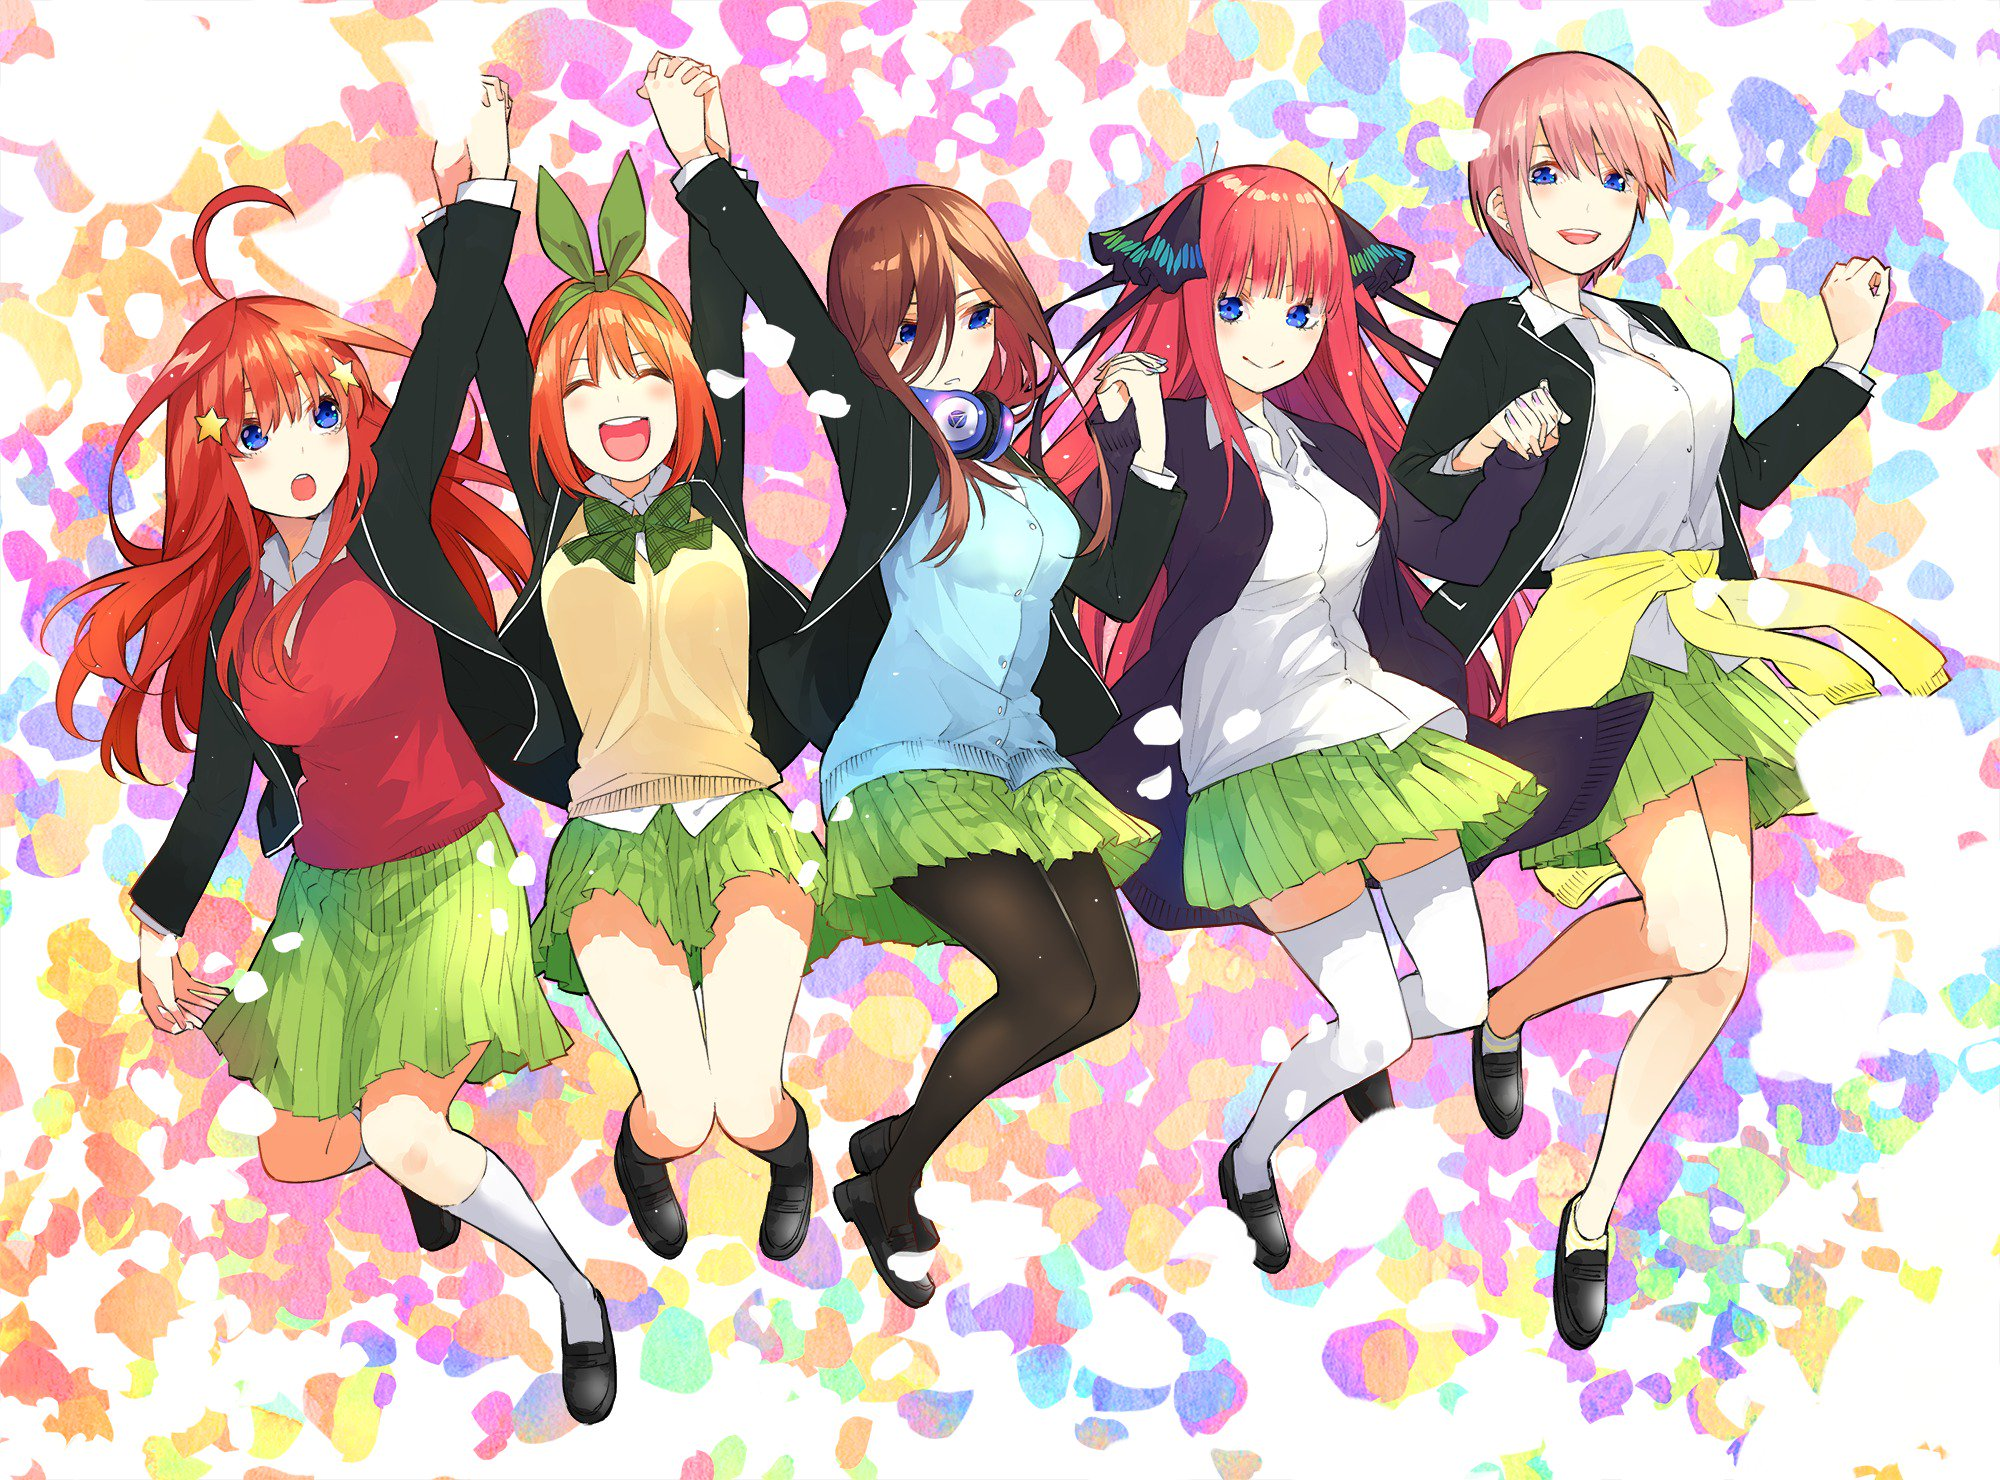
\includegraphics[clip, width=4.5cm]{./sample.jpg}
          \hspace{1.6cm} [1]通常画像
        \end{center}
      \end{minipage}

      % 2
      \begin{minipage}{0.33\hsize}
        \begin{center}
          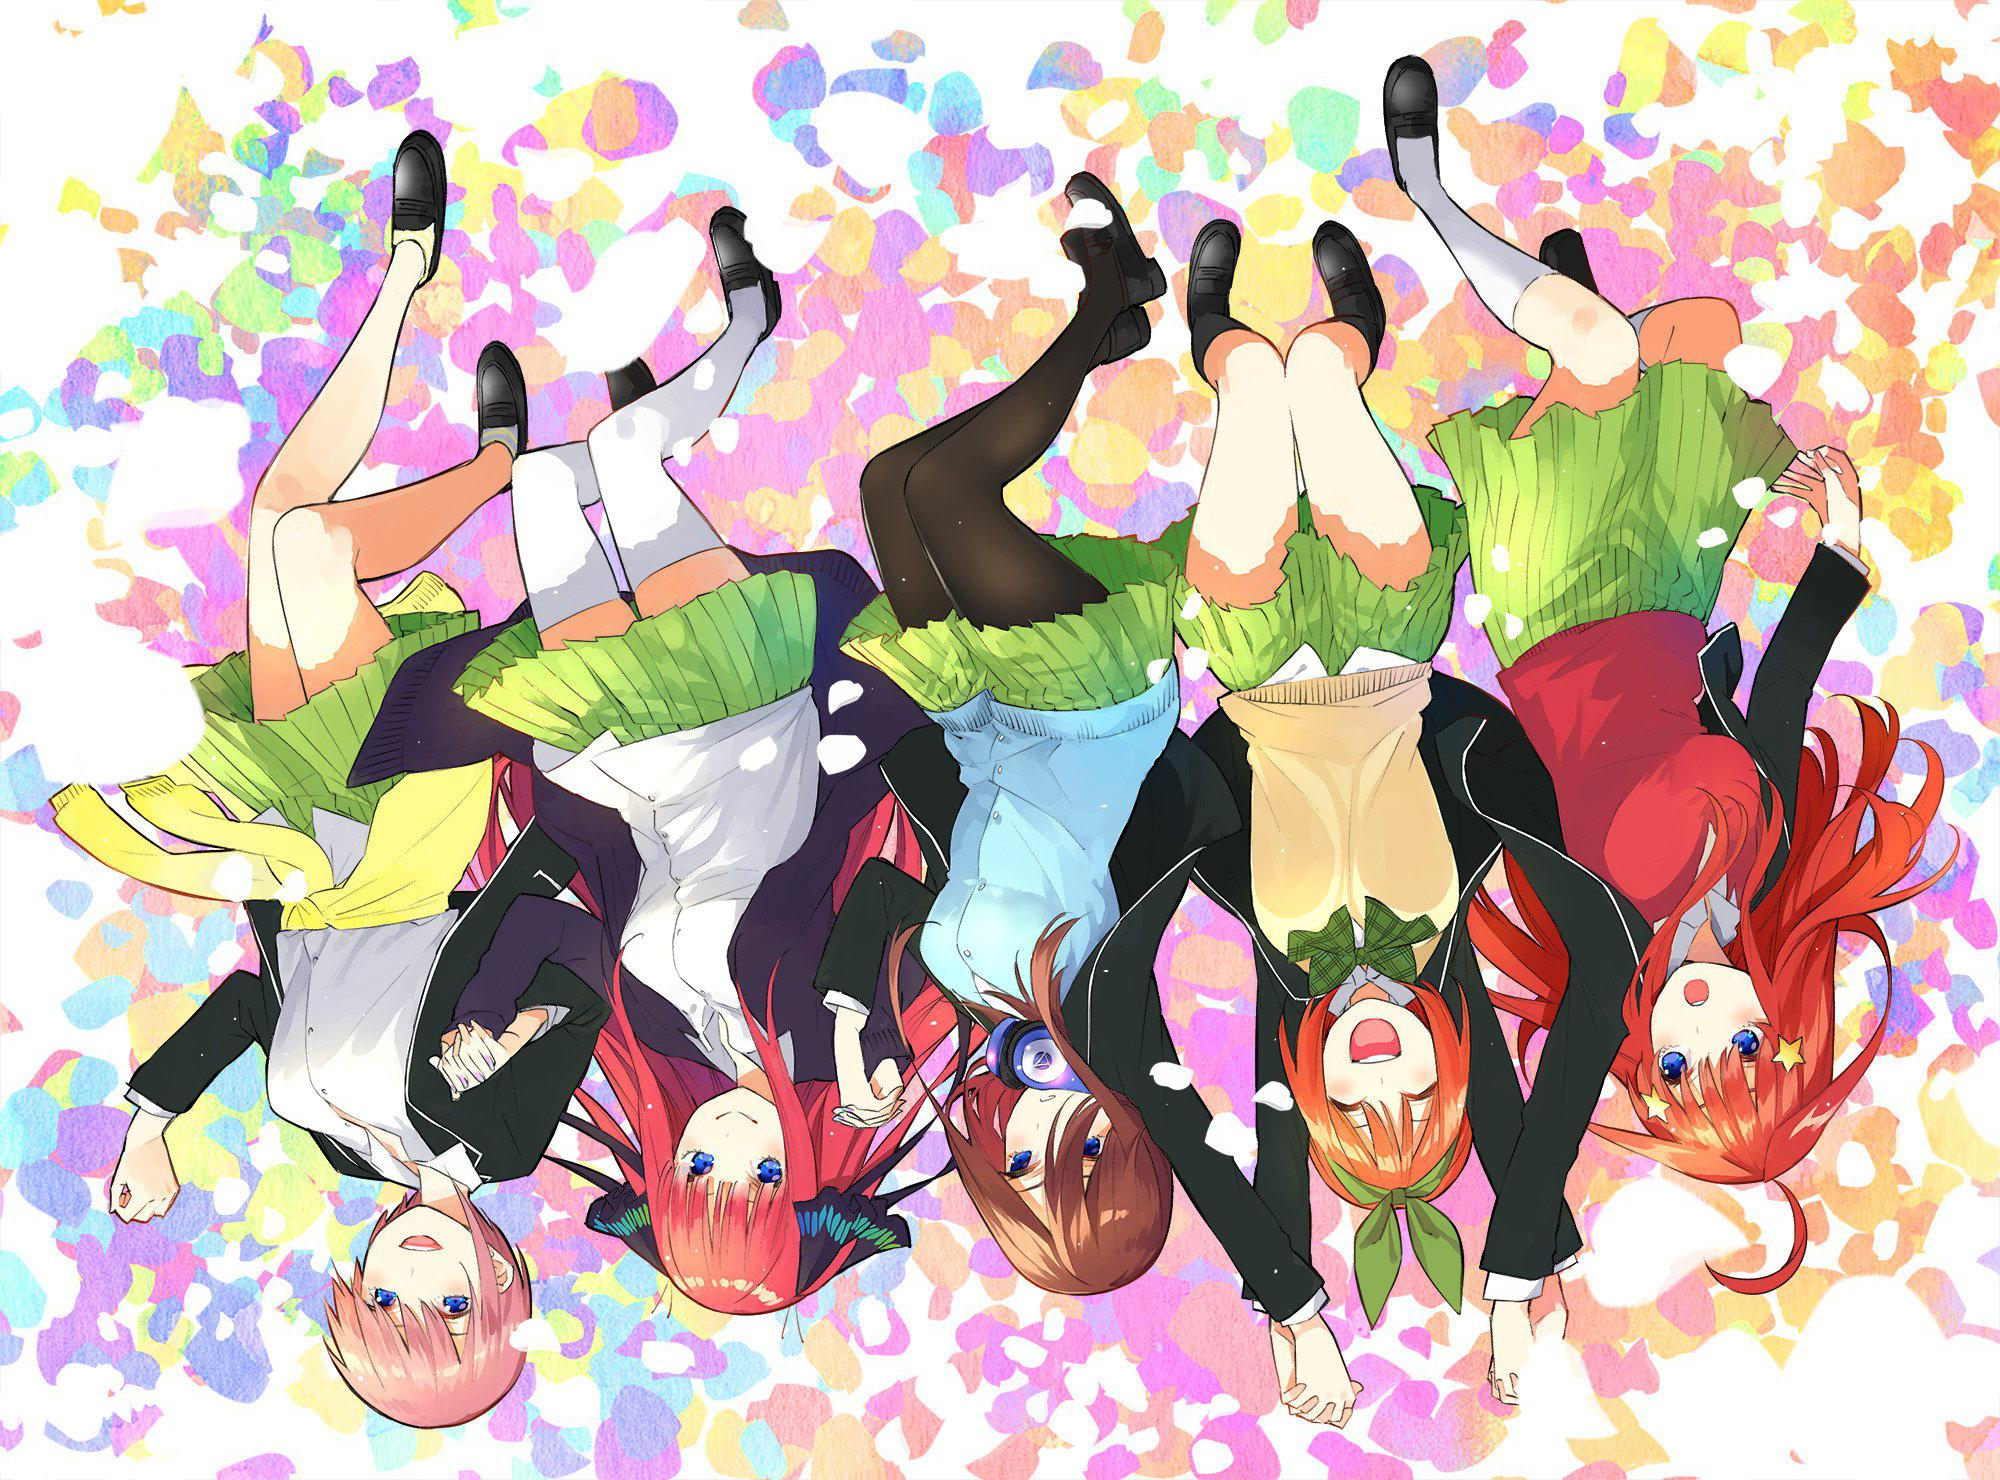
\includegraphics[clip, width=4.5cm]{./Inversdst.jpg}
          \hspace{1.6cm} [2]上下左右反転
        \end{center}
        
      \end{minipage}
       \end{tabular}
    \caption{上下左右反転}
    \label{fig:lena}
  \end{center}
\end{figure}

\section{モザイクタイル左右反転}
\subsection{ソースコード}
\lstinputlisting[language=python, numbers=left, breaklines=true, basicstyle=\ttfamily\footnotesize,
  frame=single, caption=モザイクバラバラ, label=sample]{MosaicTile.py}
\subsection{実行結果}
\clearpage
\begin{figure}
  \centering
  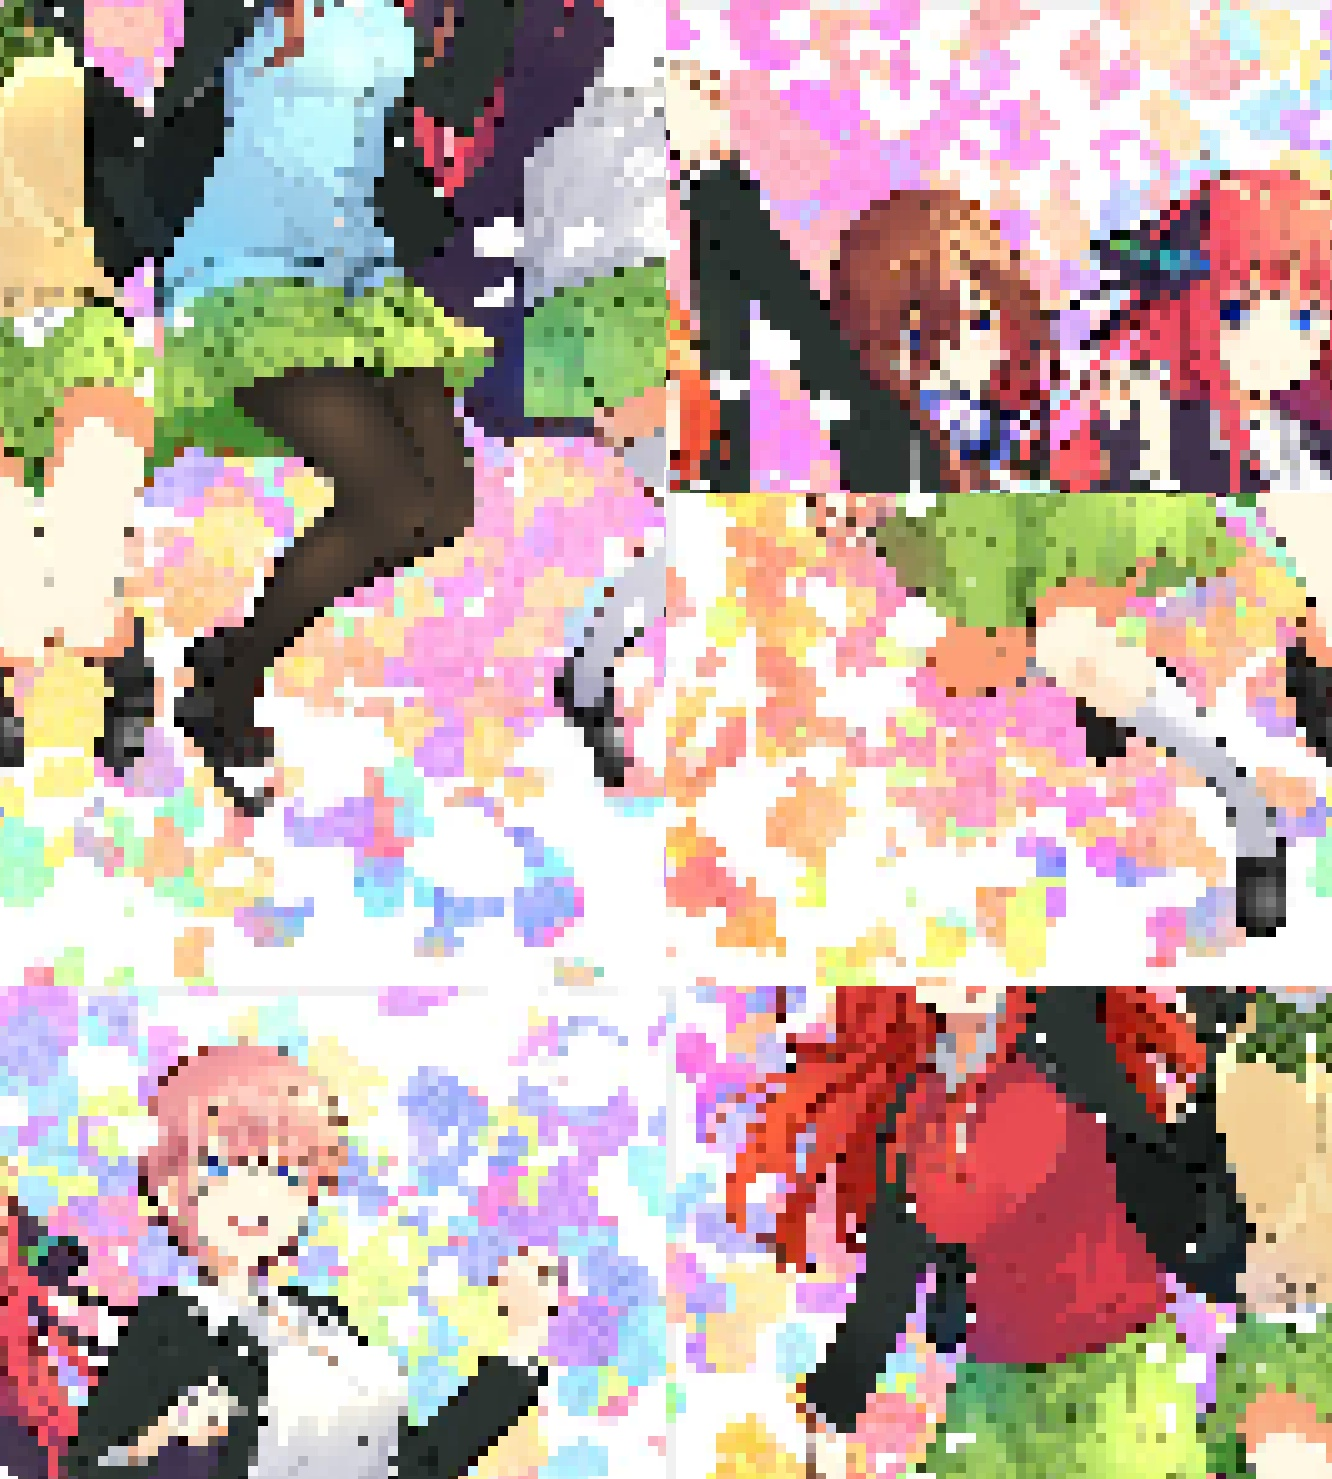
\includegraphics[width=5cm]{mosaic_result.jpg}
  \caption{実行結果}
\end{figure}

\section{平均化フィルタの調査}

\subsection{ソースコード}
\lstinputlisting[language=python, numbers=left, breaklines=true, basicstyle=\ttfamily\footnotesize,
  frame=single, caption=(3×3)の平均化フィルタ, label=sample]{Inversion.py}
\lstinputlisting[language=python, numbers=left, breaklines=true, basicstyle=\ttfamily\footnotesize,
  frame=single, caption=(5×5)の平均化フィルタ, label=sample]{Inversion.py}
\lstinputlisting[language=python, numbers=left, breaklines=true, basicstyle=\ttfamily\footnotesize,
  frame=single, caption=(3×3)の加重平均化フィルタ, label=sample]{Inversion.py}
\lstinputlisting[language=python, numbers=left, breaklines=true, basicstyle=\ttfamily\footnotesize,
  frame=single, caption=(5×5)の加重平均化フィルタ, label=sample]{Inversion.py}

\subsection{実行結果}
\begin{figure}[htpb]
  \centering
    \begin{tabular}{c}
 
%----- y = sin(x) -----
 
      \begin{minipage}{0.47\hsize}
        \centering
          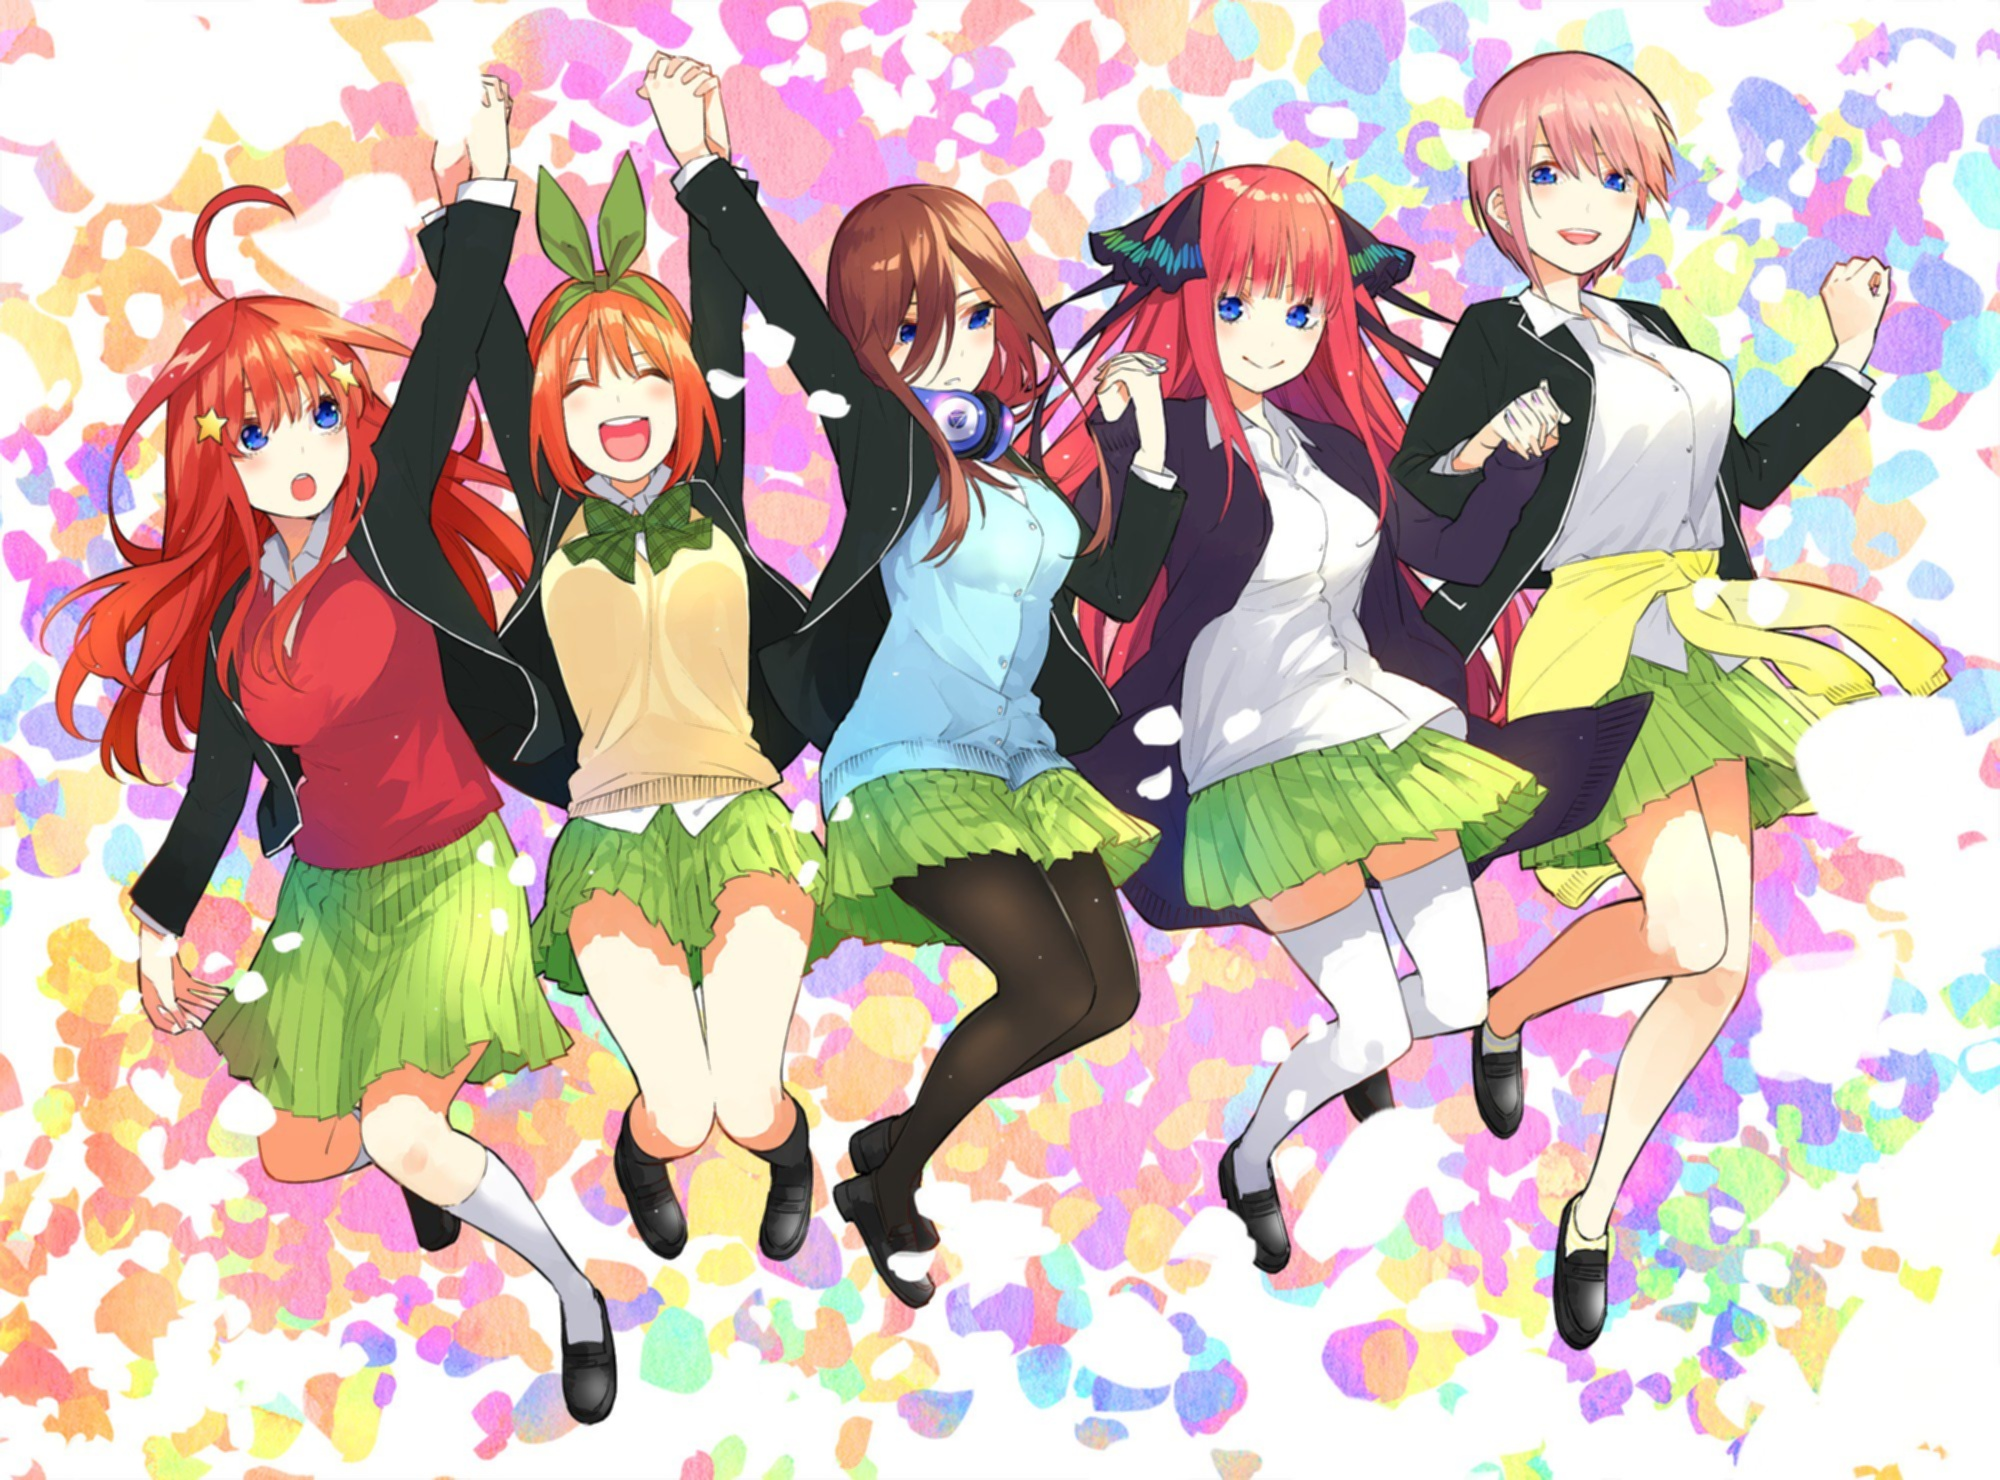
\includegraphics[keepaspectratio, scale=0.07, angle=0]
                          {output5_1.jpg}
                          \caption{(3×3)の平均化フィルタ}
                          \label{fig:sin_x}
      \end{minipage}
 
%--- 中央スペース
 
      \begin{minipage}{0.06\hsize}
        \hspace{2mm}
      \end{minipage}
 
%----- y = sin(2x) -----
 
      \begin{minipage}{0.47\hsize}
        \centering
          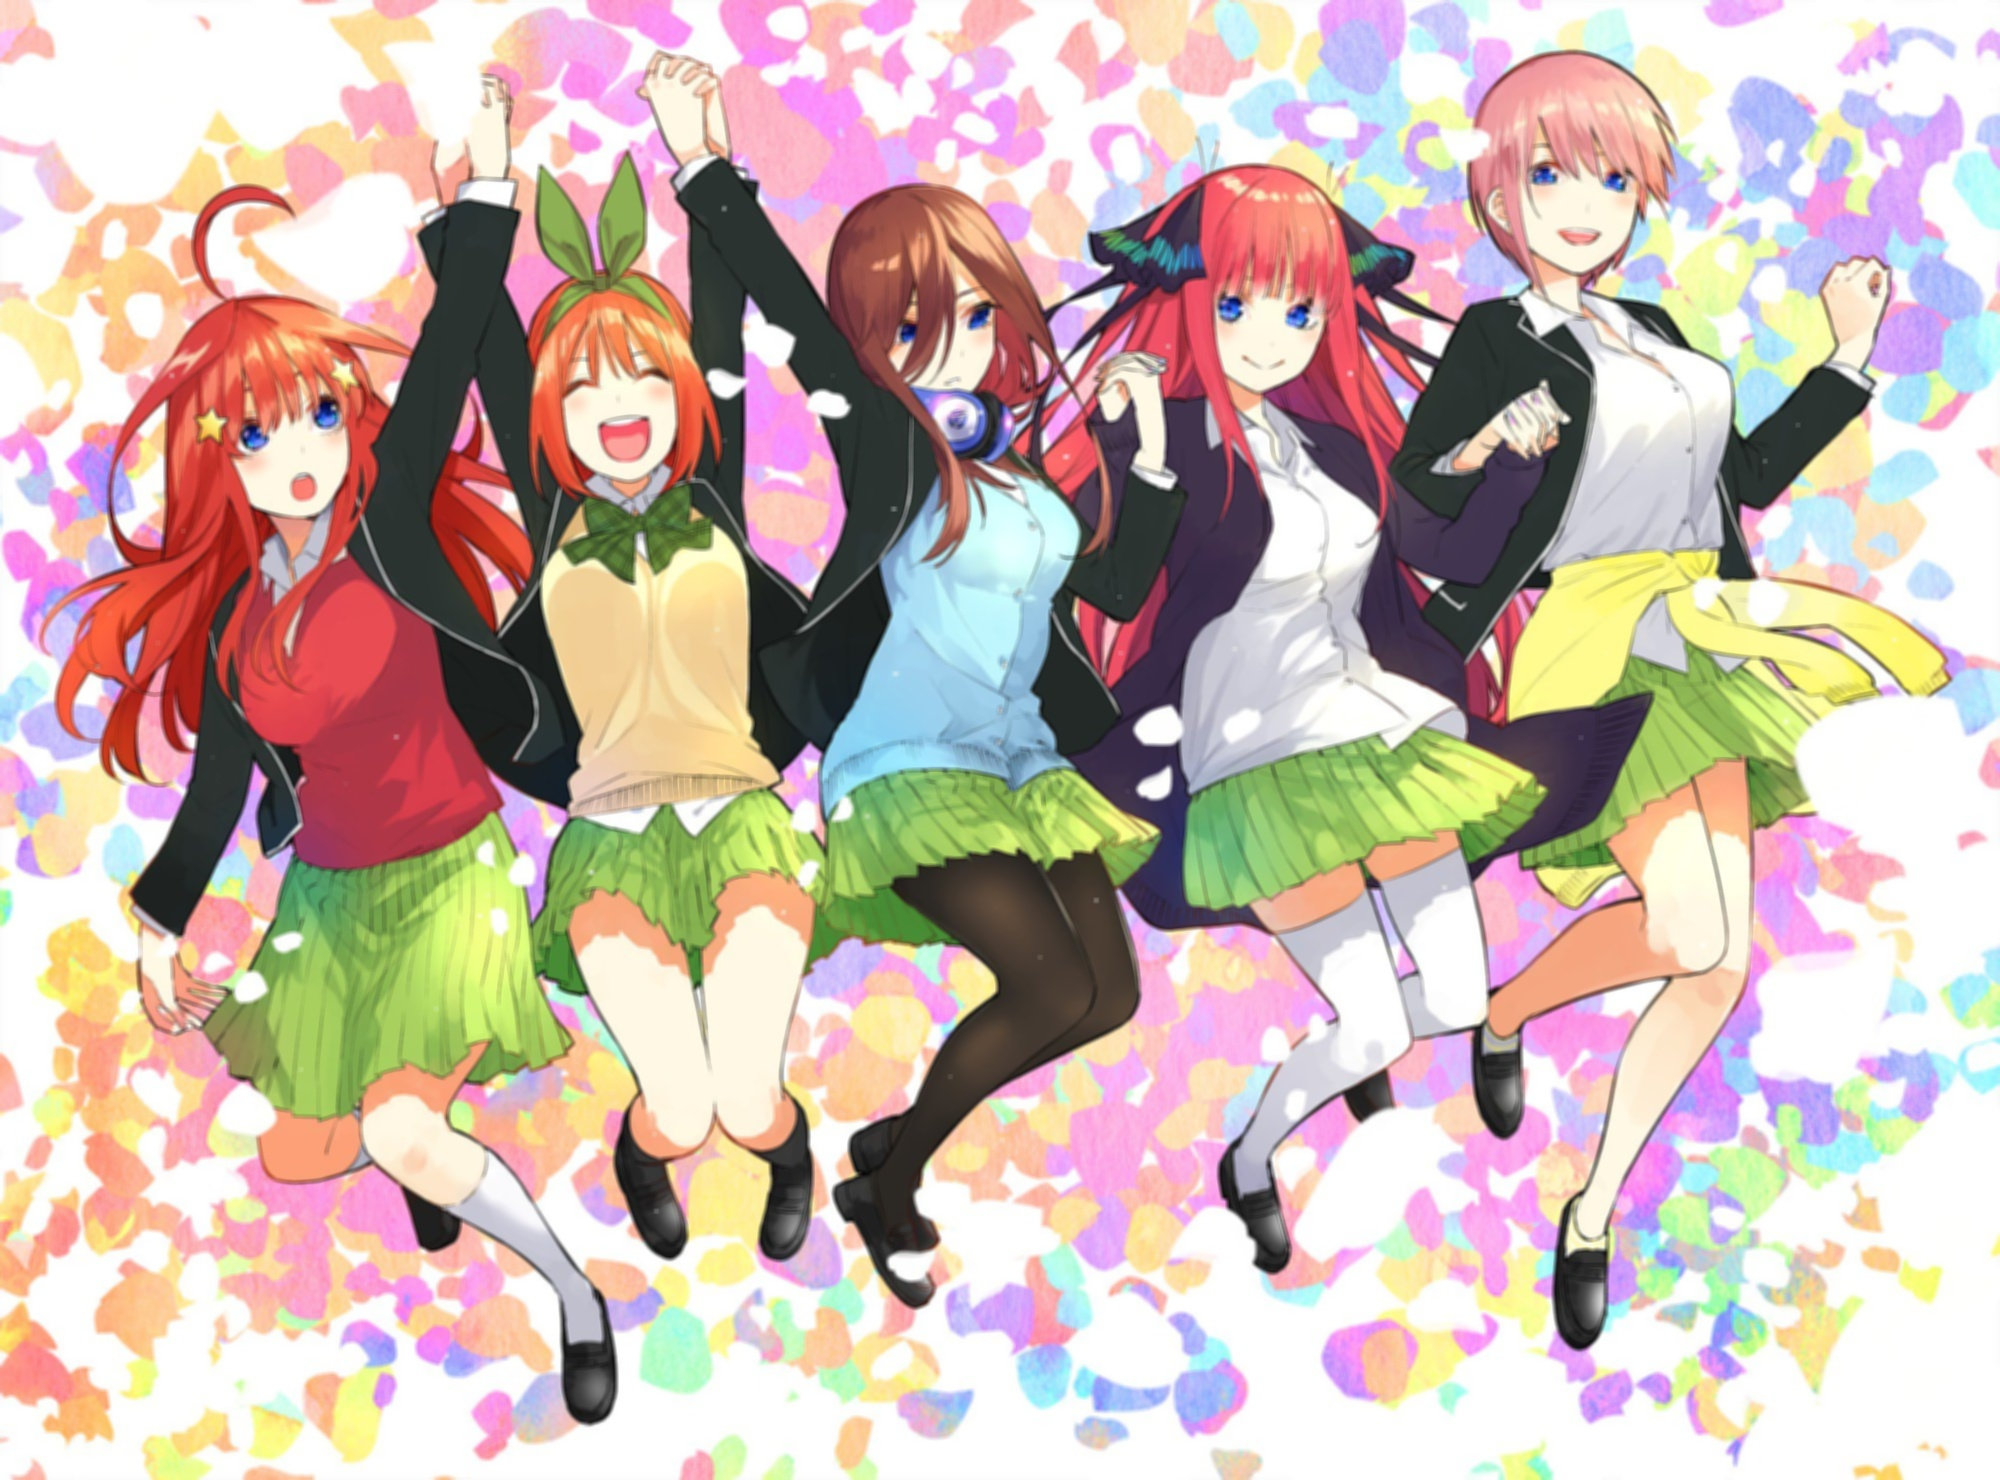
\includegraphics[keepaspectratio, scale=0.07, angle=0]
                          {output5_2.jpg}
                          \caption{(5×5)の平均化フィルタ}
                          \label{fig:sin_2x}
      \end{minipage} \\
 
%--- 上下スペース
 
      \begin{minipage}{0.06\hsize}
        \vspace{10mm}
      \end{minipage} \\
 
 
%----- y = sin(3x) -----
 
      \begin{minipage}{0.47\hsize}
        \centering
          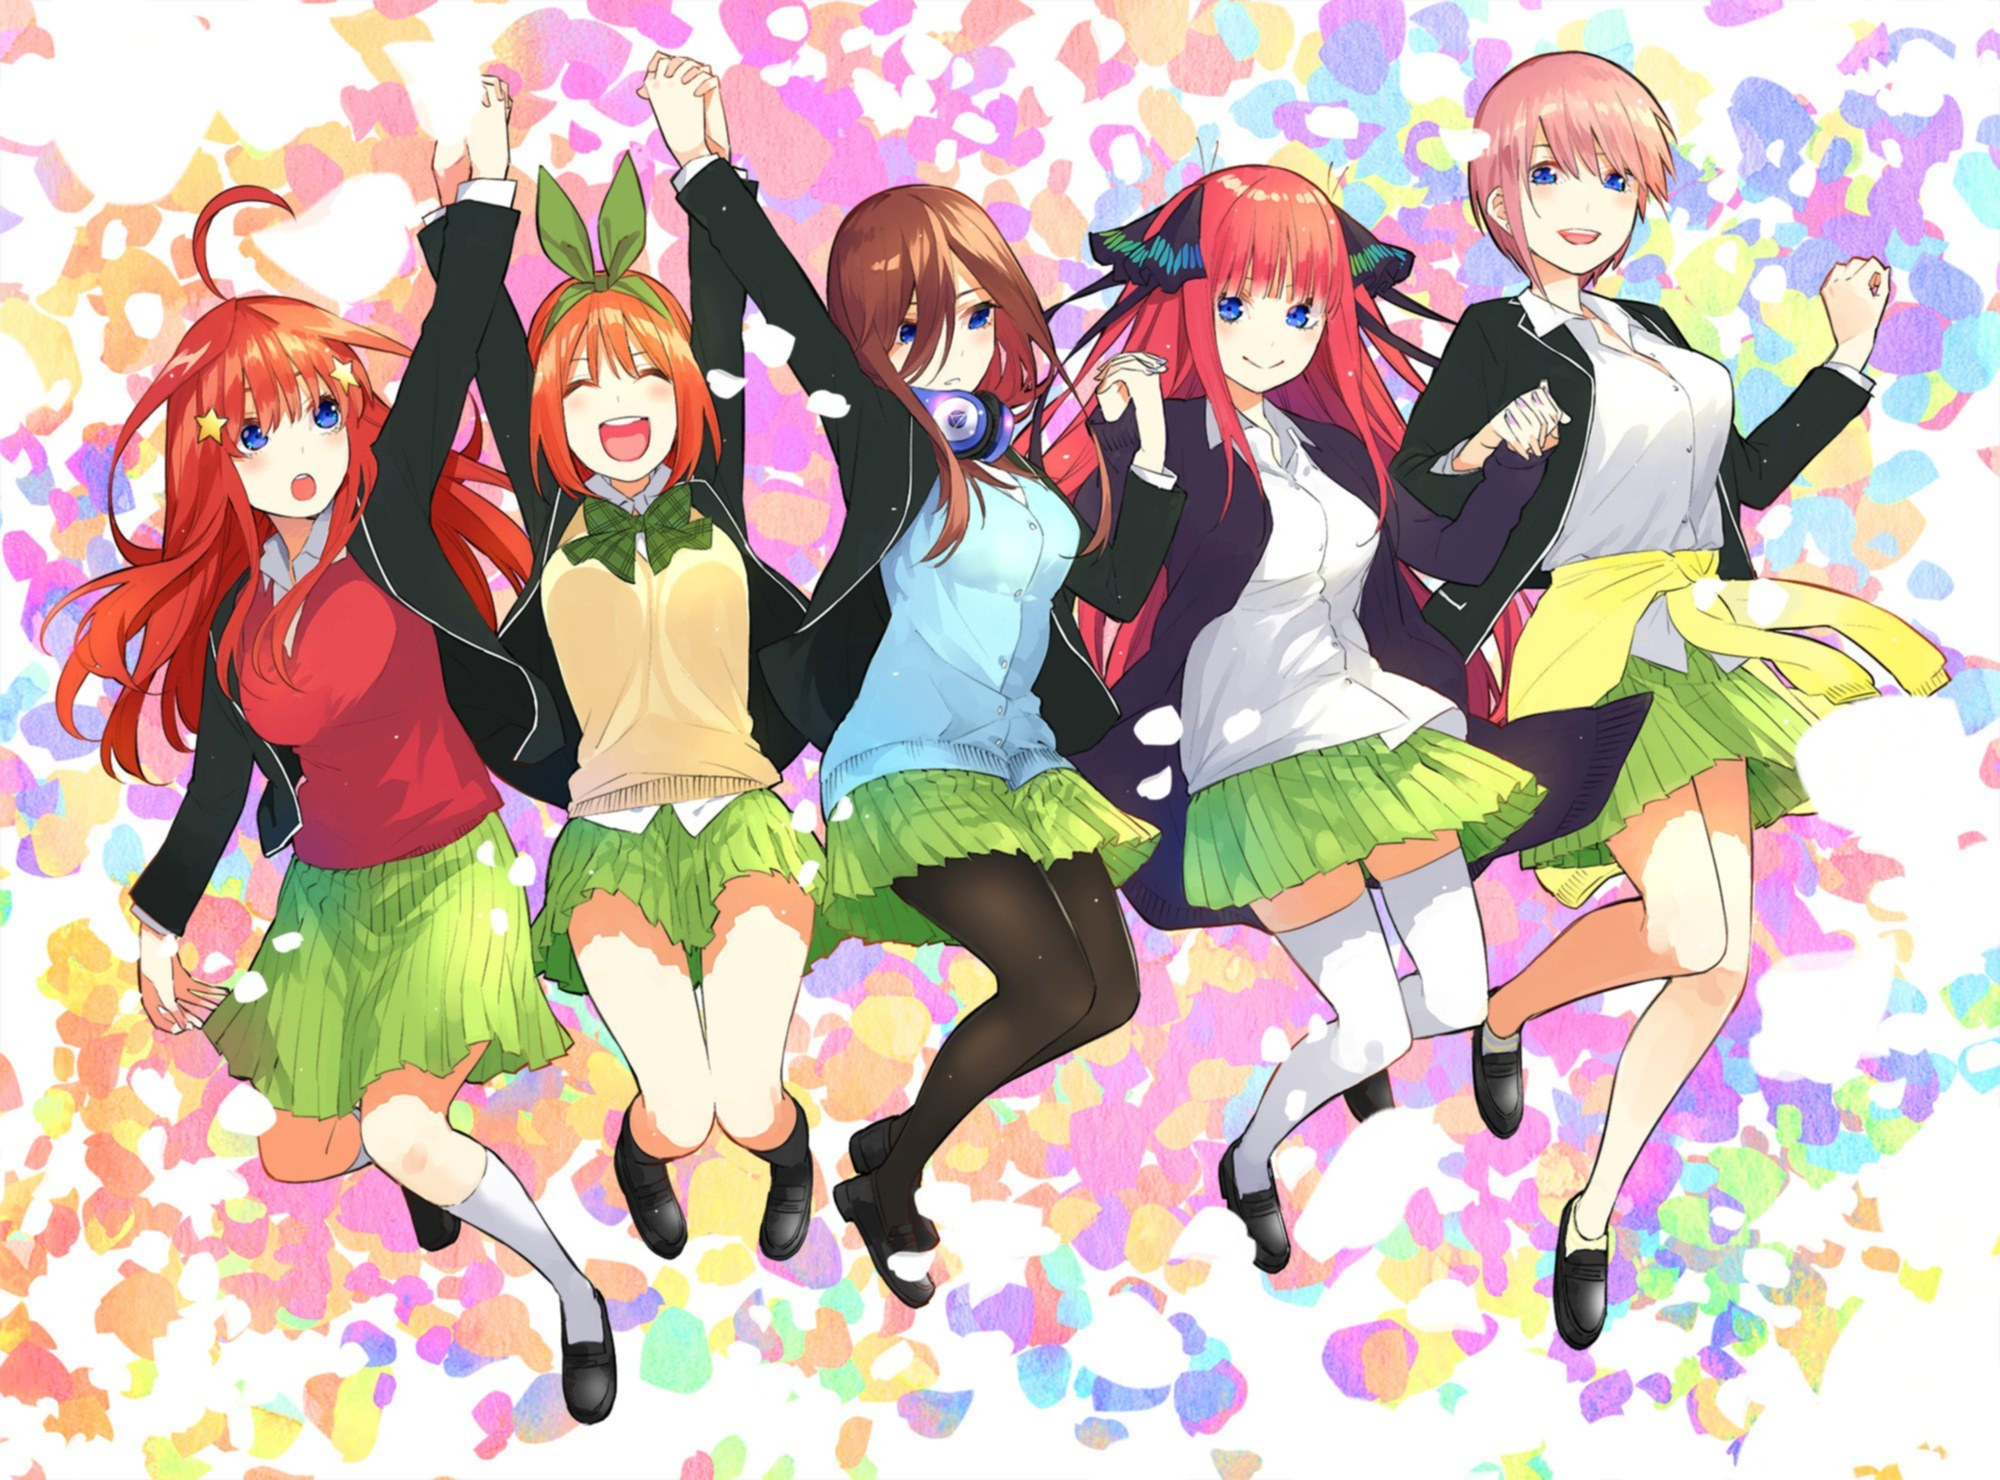
\includegraphics[keepaspectratio, scale=0.07, angle=0]
                          {output5_3.jpg}
                          \caption{(3×3)の加重平均化フィルタ}
                          \label{fig:sin_3x}
      \end{minipage}
 
%--- 中央スペース
 
      \begin{minipage}{0.06\hsize}
        \hspace{2mm}
      \end{minipage}
 
 
%----- y = sin(4x) -----
 
      \begin{minipage}{0.47\hsize}
        \centering
          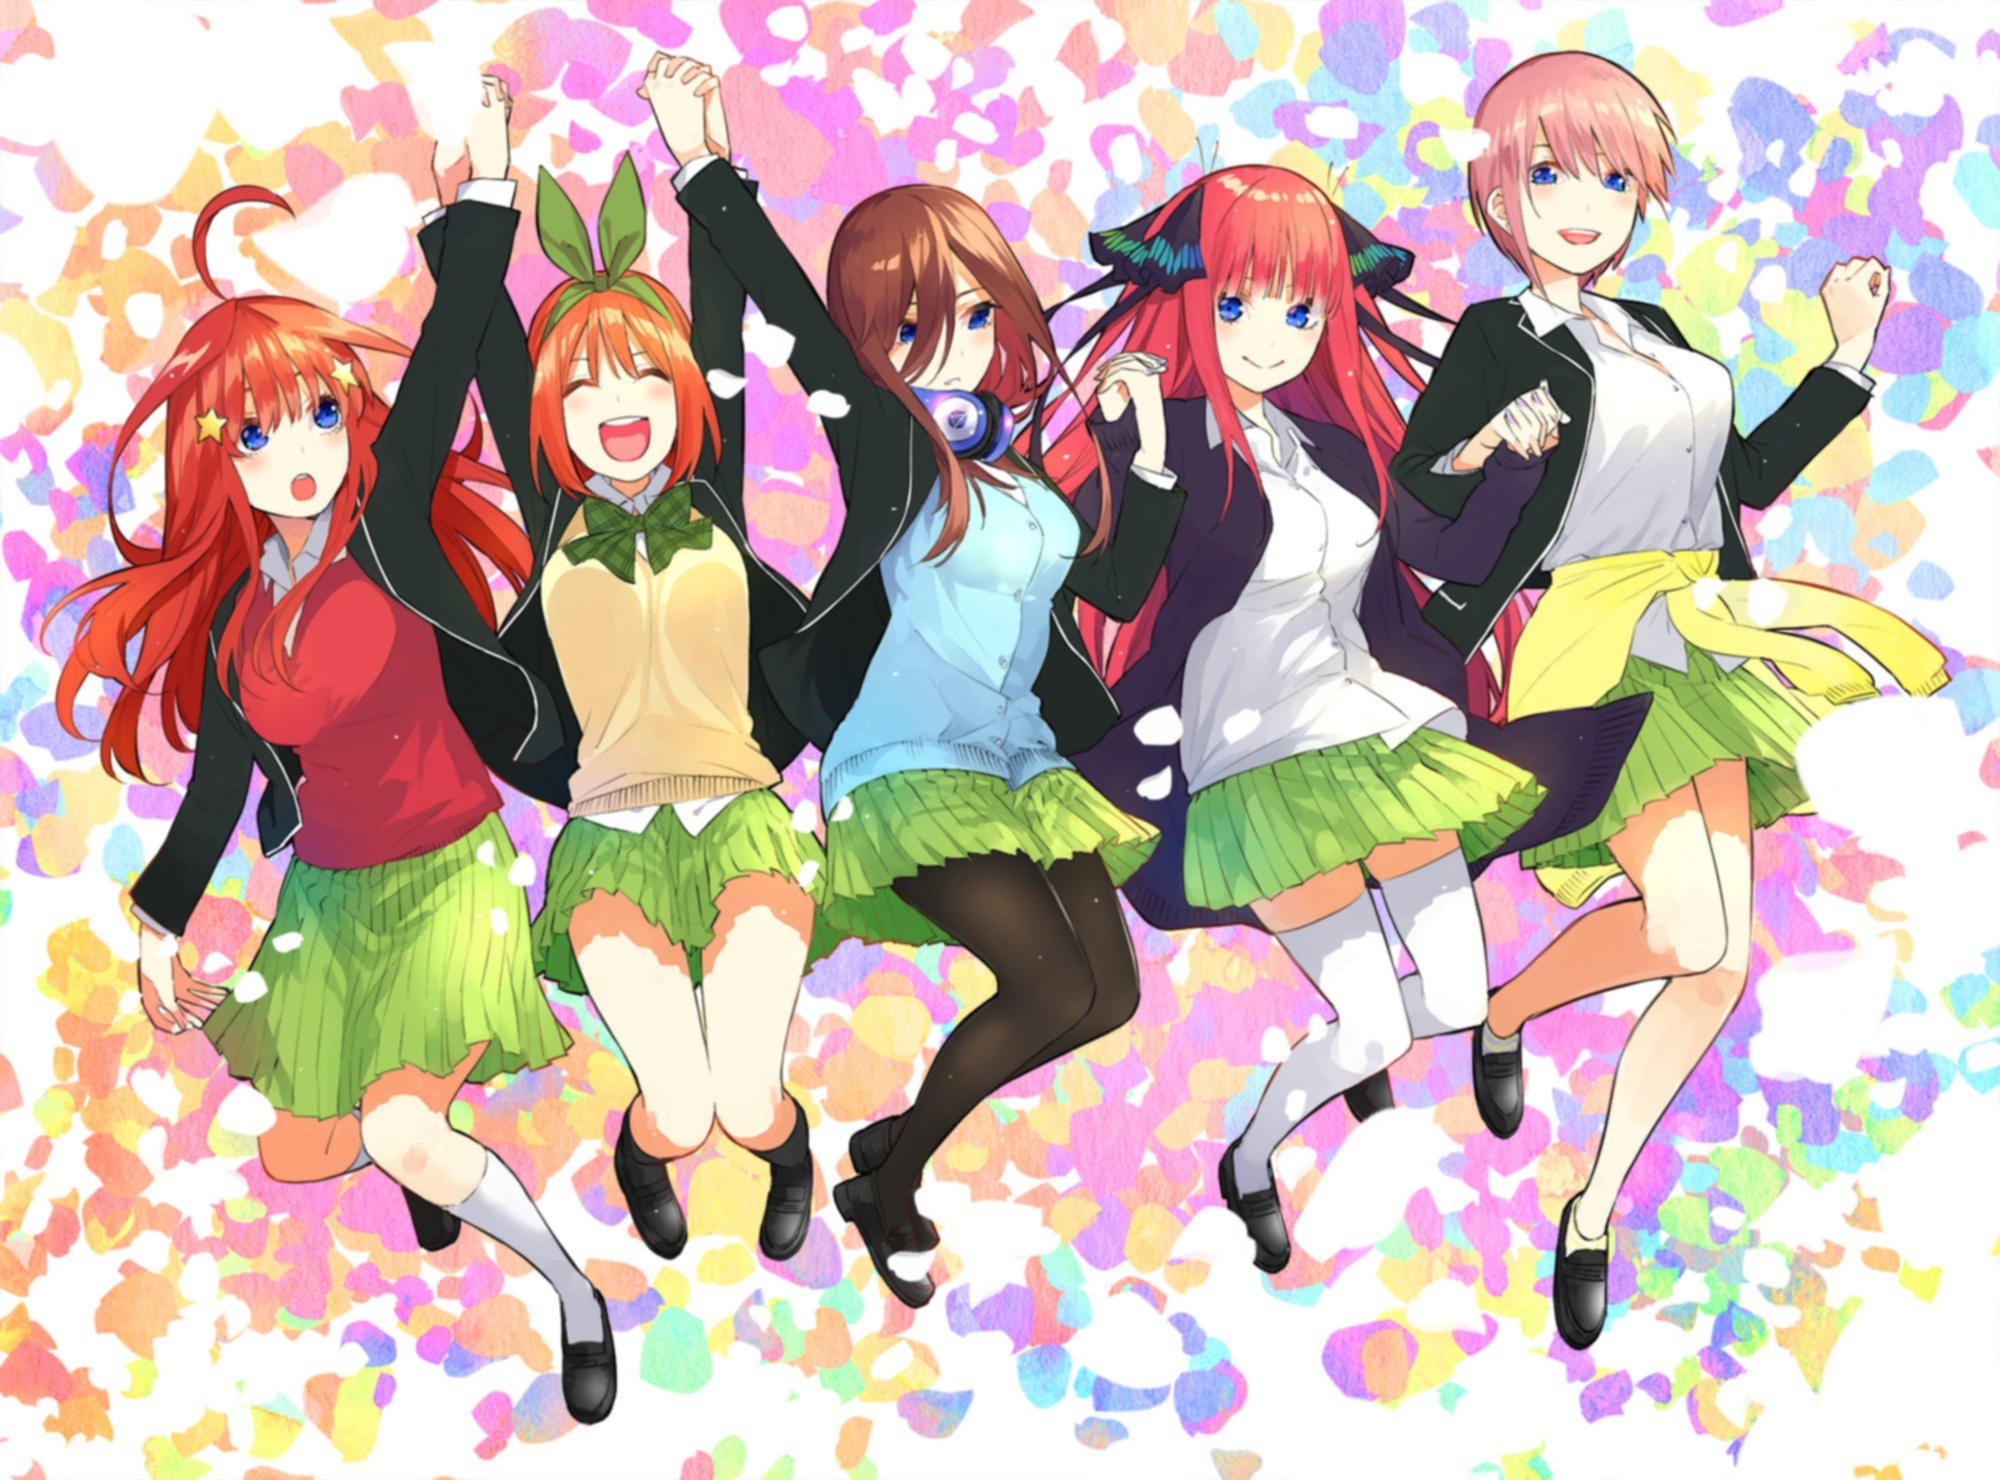
\includegraphics[keepaspectratio, scale=0.07, angle=0]
                          {output5_4.jpg}
                          \caption{(5×5)の加重平均化フィルタ}
                          \label{fig:sin_4x}
      \end{minipage}
 
 
    \end{tabular}
\end{figure}          

\subsection{考察}
平均化のフィルタのサイズが、大きくなれば色合いが良くなっているように感じられる。
荷重平均化と平均化のフィルタの違いはこの画像を見れば、違いがわからない。

\section{鮮鋭化フィルタの調査}

\subsection{ソースコード}
\lstinputlisting[language=python, numbers=left, breaklines=true, basicstyle=\ttfamily\footnotesize,
  frame=single, caption=輪郭抽出, label=sample]{SharpeningFilter.py}
\subsection{実行結果}
\begin{figure}[htbp]
  \begin{center}
    \begin{tabular}{c}

      % 1
      \begin{minipage}{0.33\hsize}
        \begin{center}
          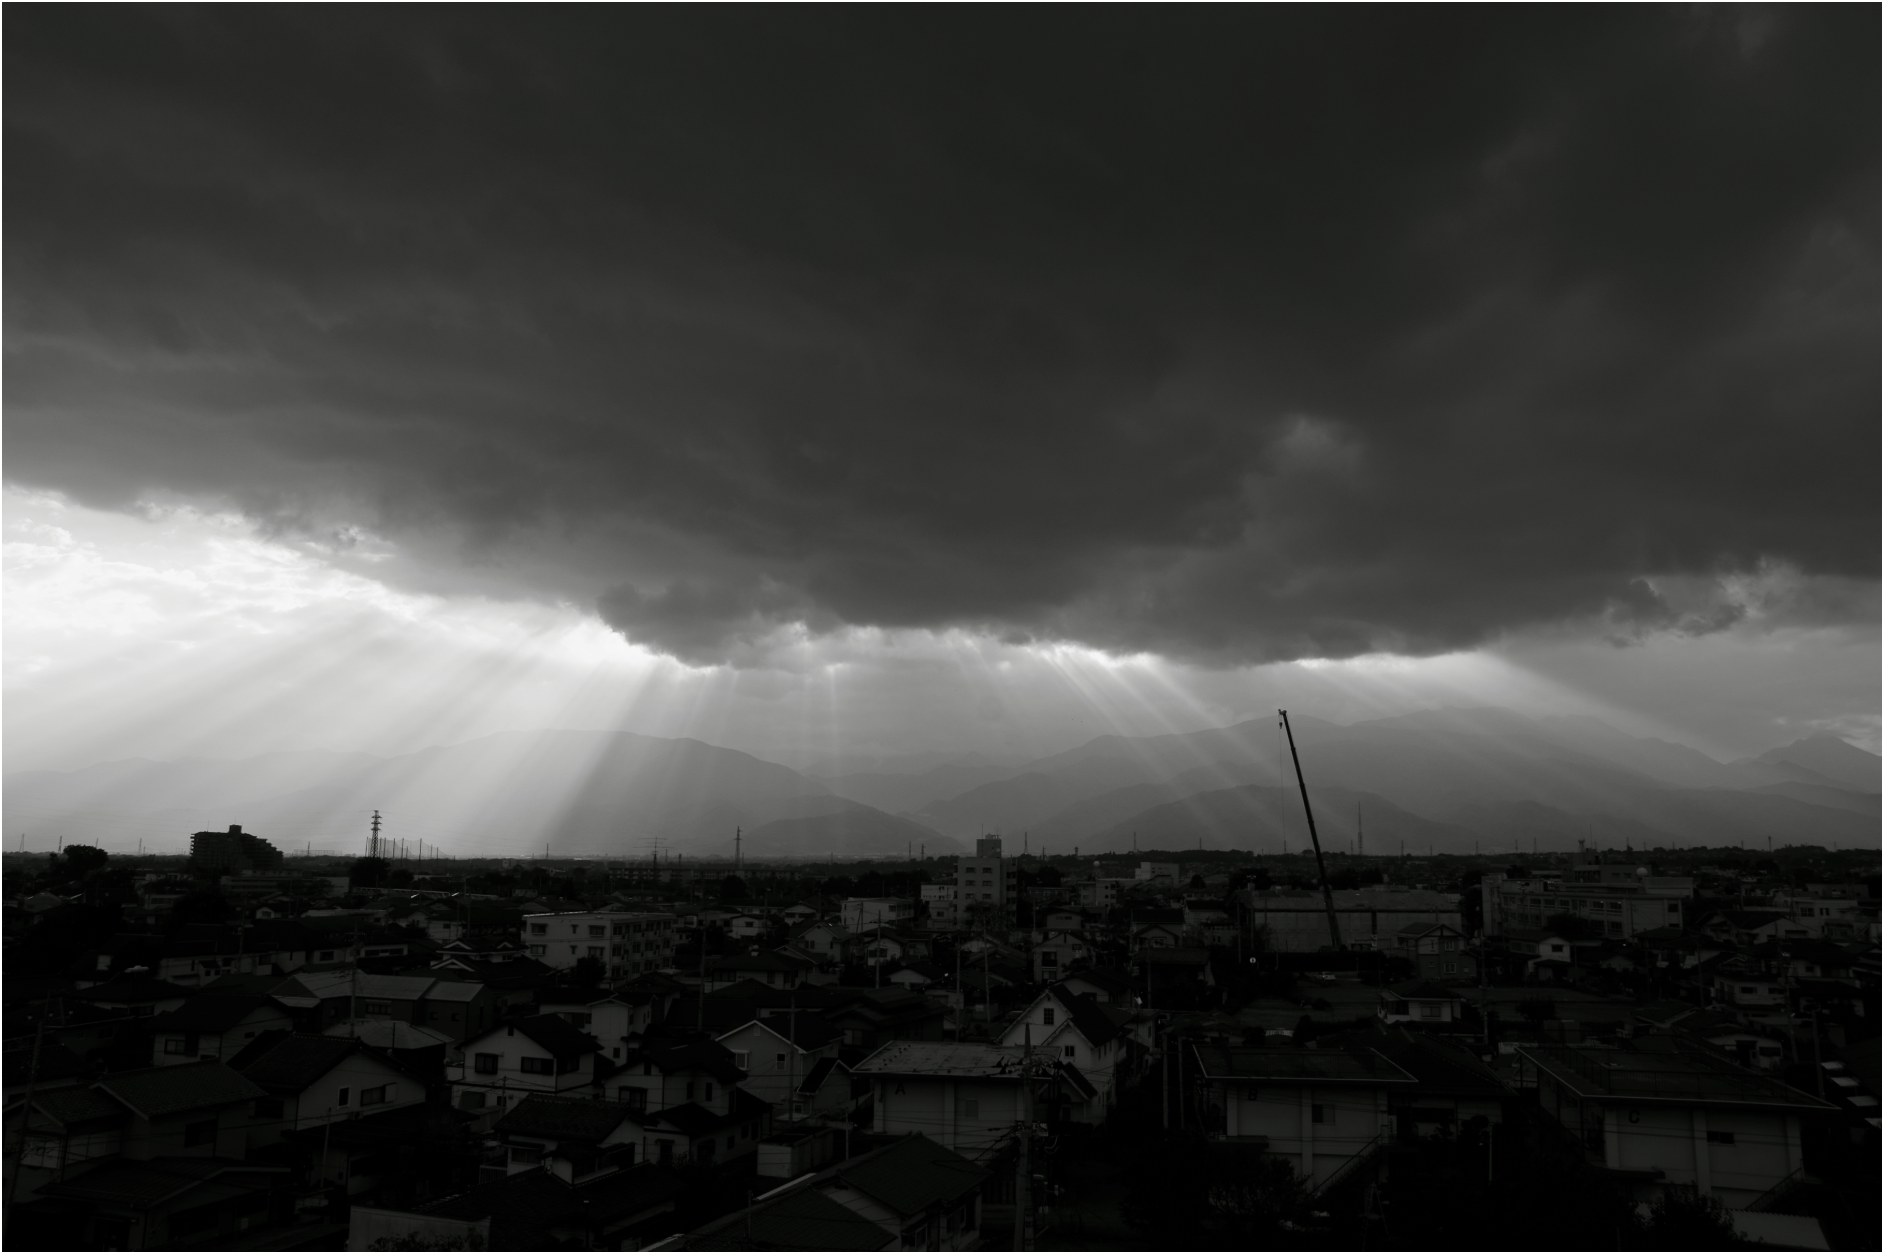
\includegraphics[clip, width=4.5cm]{./sample2.jpg}
          \hspace{1.6cm} [1]通常画像
        \end{center}
      \end{minipage}

      % 2
      \begin{minipage}{0.33\hsize}
        \begin{center}
          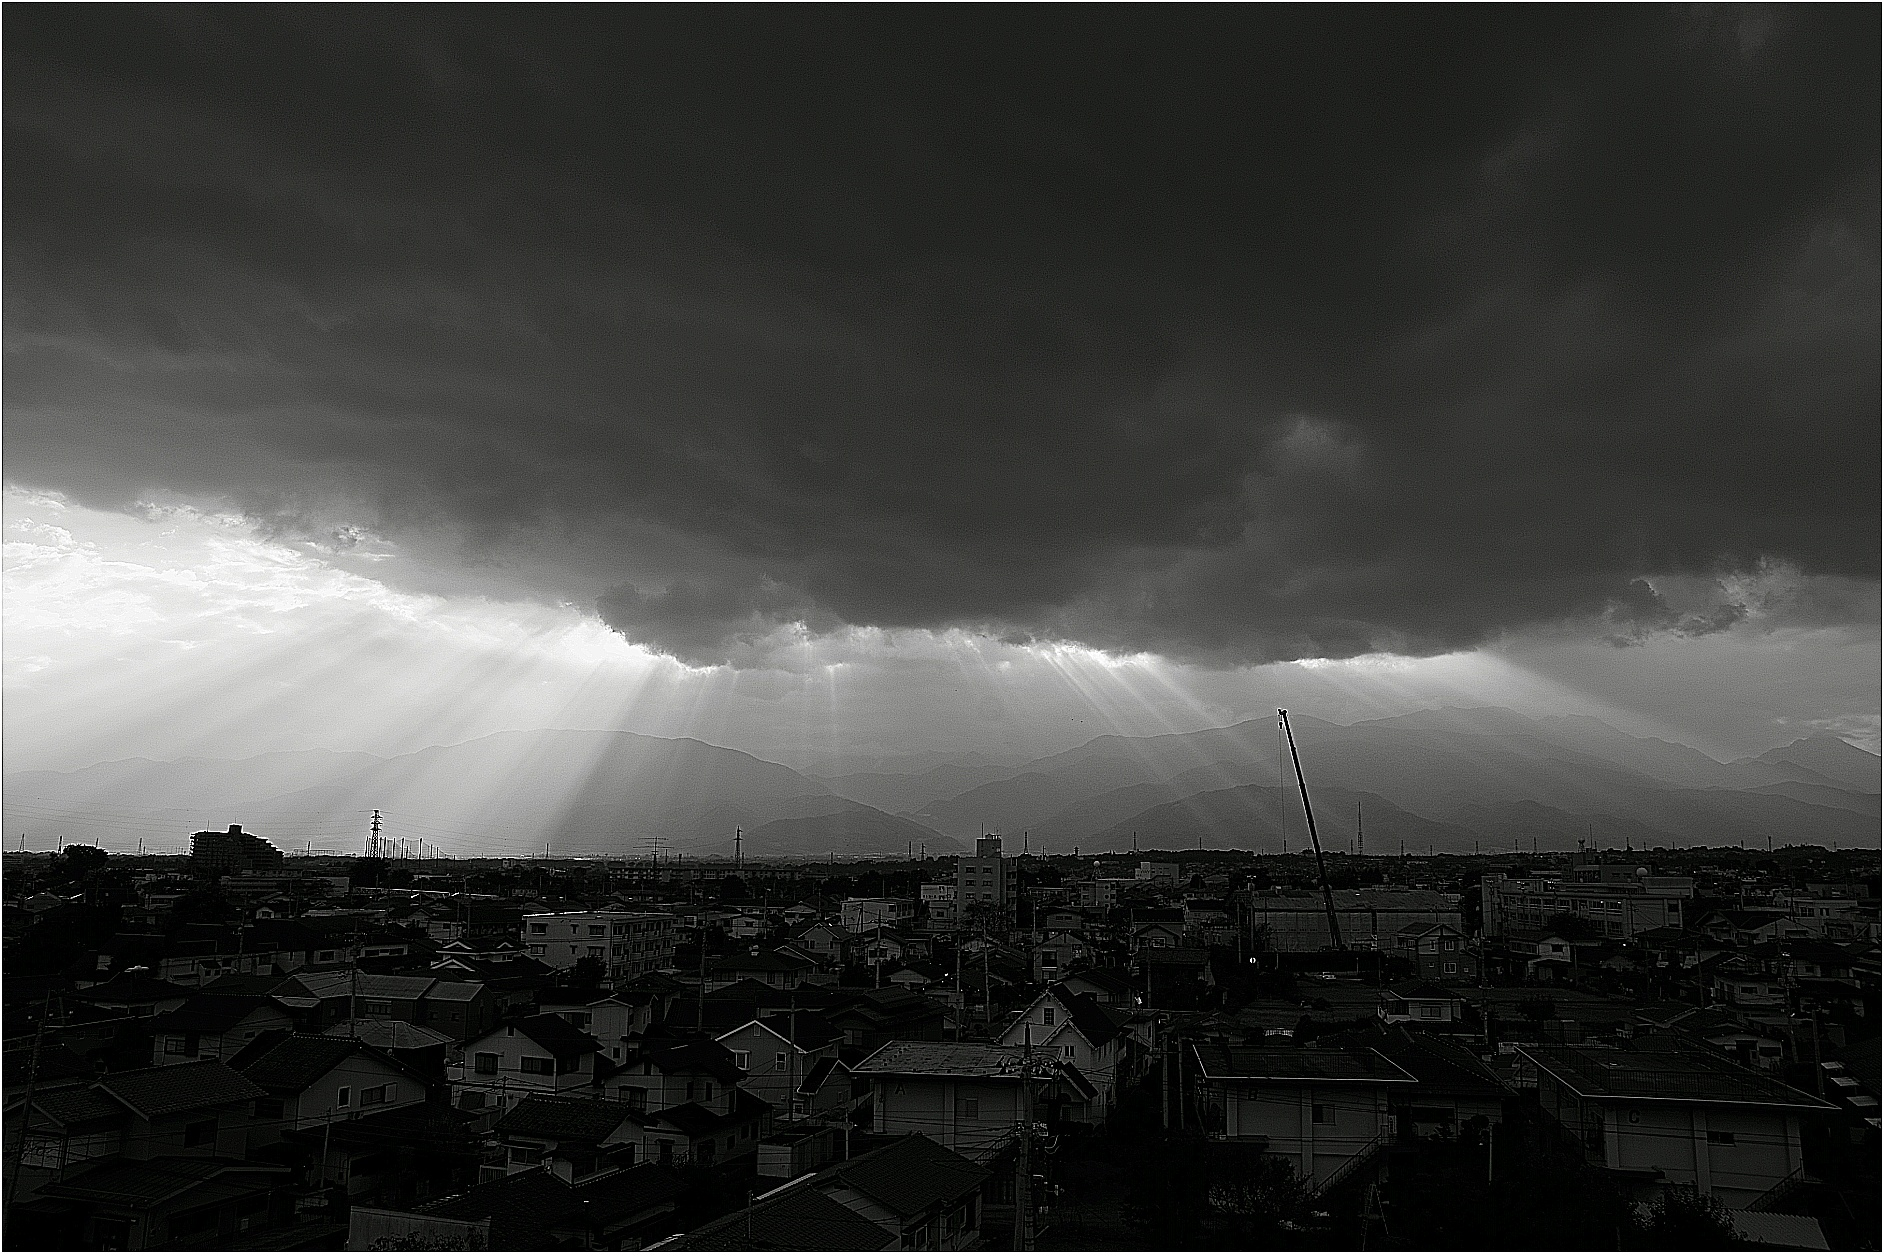
\includegraphics[clip, width=4.5cm]{./output6.jpg}
          \hspace{1.6cm} [2]ganm=1.5
        \end{center}
      \end{minipage}

      % 3
      \begin{minipage}{0.33\hsize}
        \begin{center}
          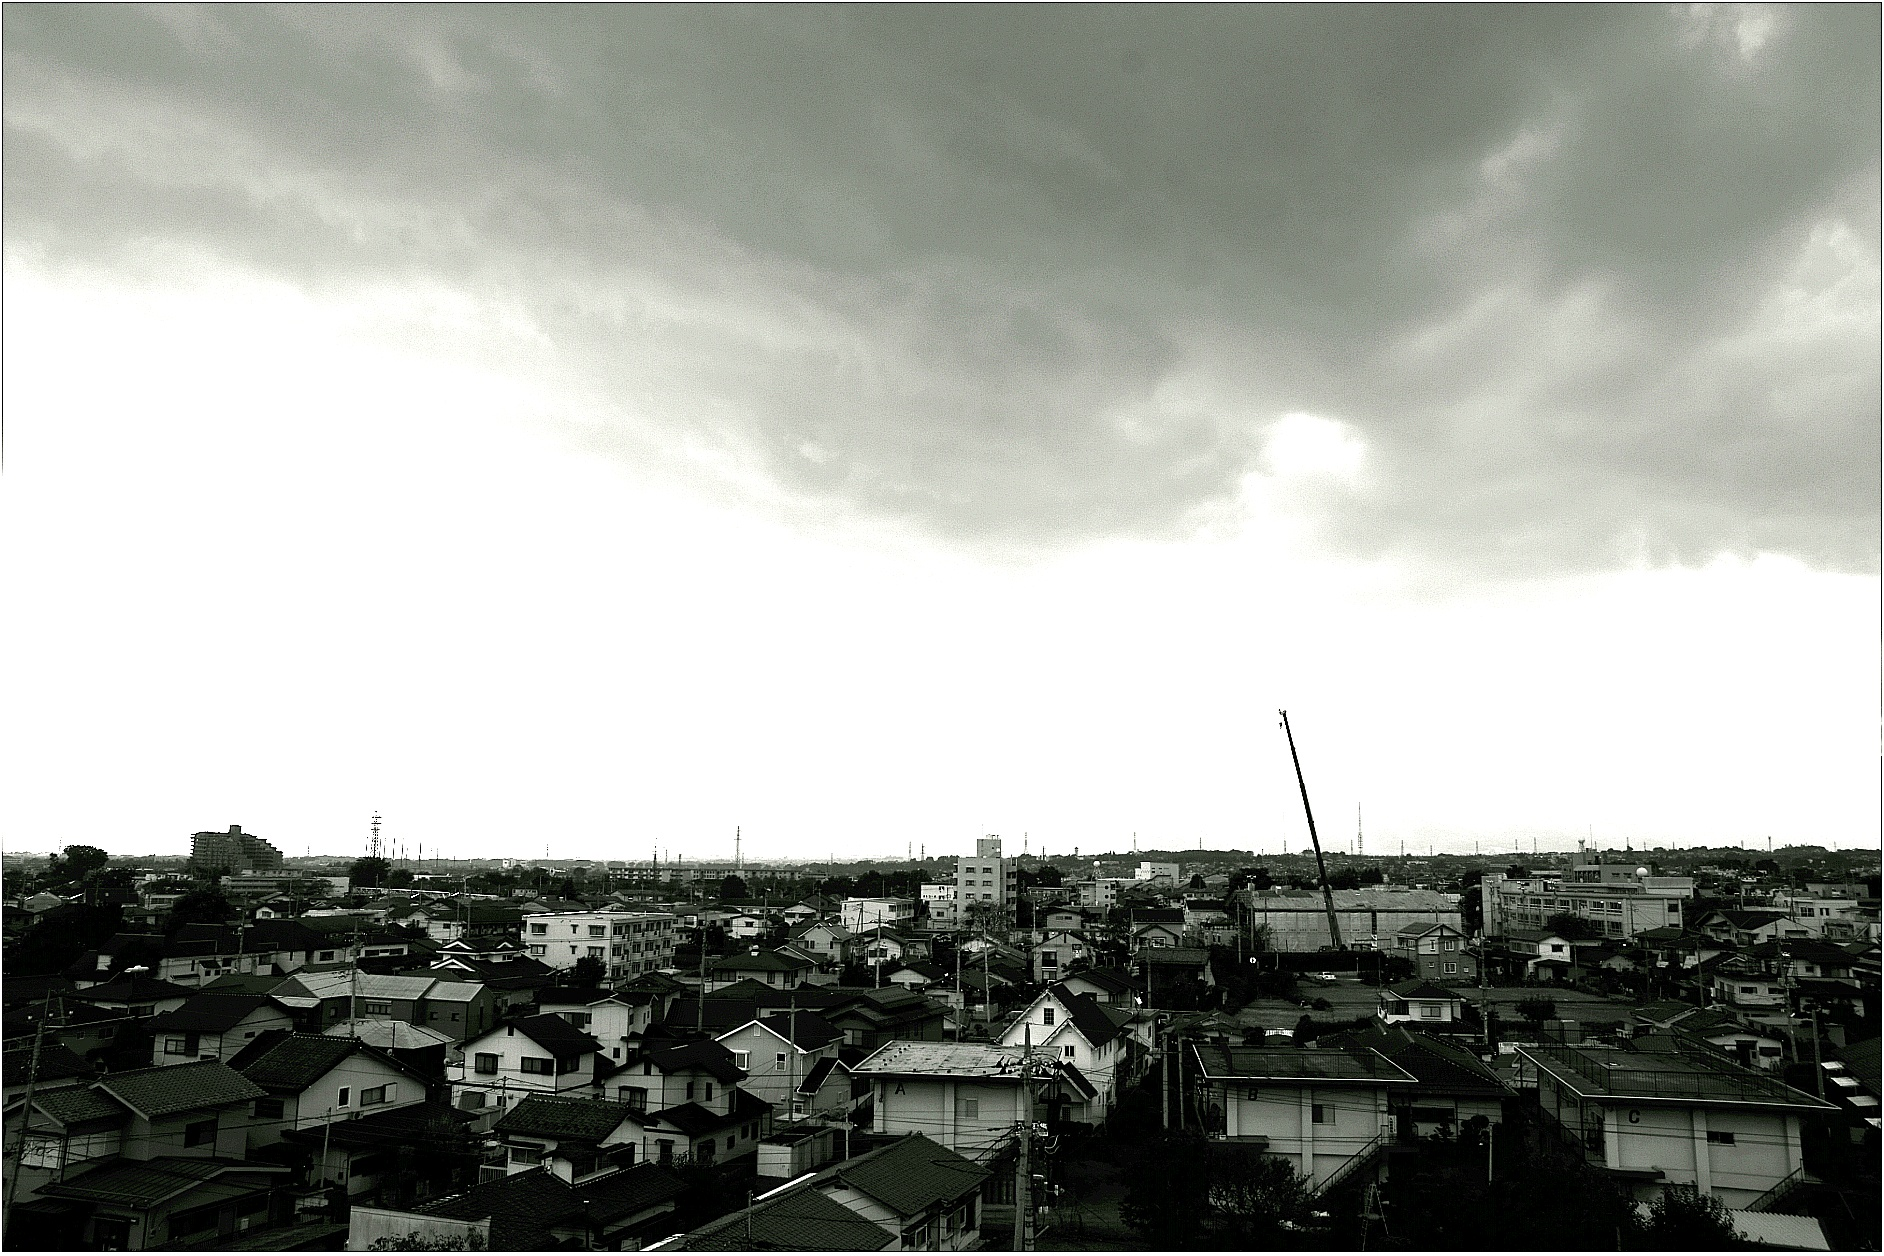
\includegraphics[clip, width=4.5cm]{./output6_1.jpg}
          \hspace{1.6cm} [3]ganm=0.5
        \end{center}
      \end{minipage}

    \end{tabular}
    \caption{トーンカーブ}
    \label{fig:lena}
  \end{center}
\end{figure}

\subsection{考察}
ganmの値を大きくすると画像全体が暗くなってしまい、値を小さくすると明るくなり、見えずらかった、町が見やすくなった

\section{輪郭抽出}
\subsection{ソースコード}
\lstinputlisting[language=python, numbers=left, breaklines=true, basicstyle=\ttfamily\footnotesize,
  frame=single, caption=輪郭抽出, label=sample]{ContourExtraction.py}
\subsection{実行結果}
\begin{figure}[htbp]
  \begin{center}
    \begin{tabular}{c}
      % 1
      \begin{minipage}{0.33\hsize}
        \begin{center}
          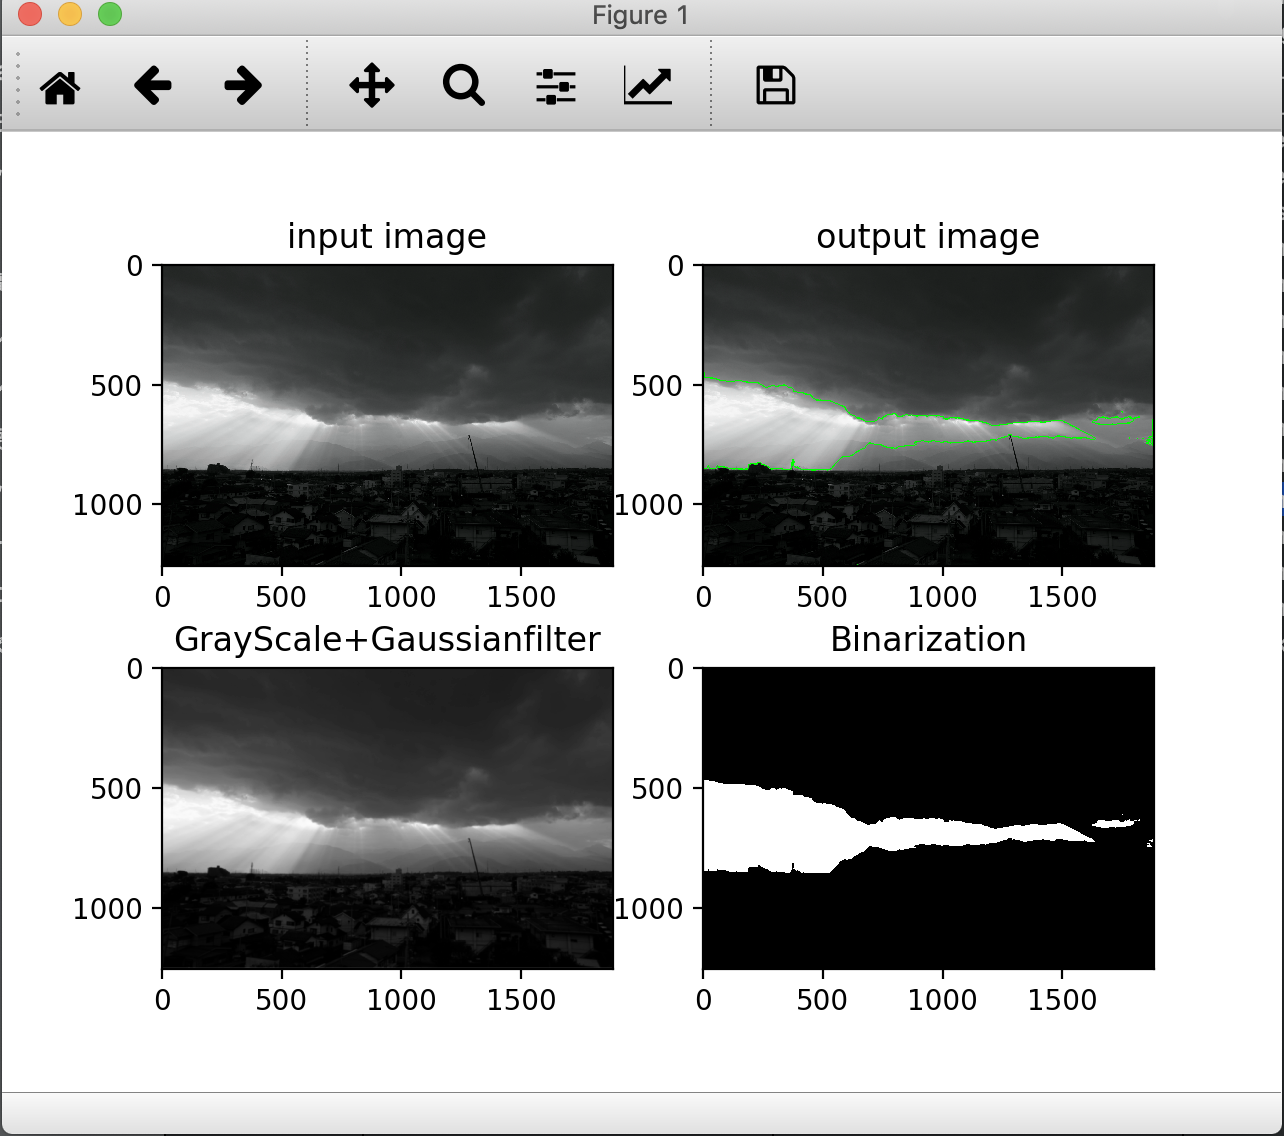
\includegraphics[clip, width=4.5cm]{./output1.png}
          \hspace{1.6cm} [1]結果画像その1
        \end{center}
      \end{minipage}

      % 2
      \begin{minipage}{0.33\hsize}
        \begin{center}
          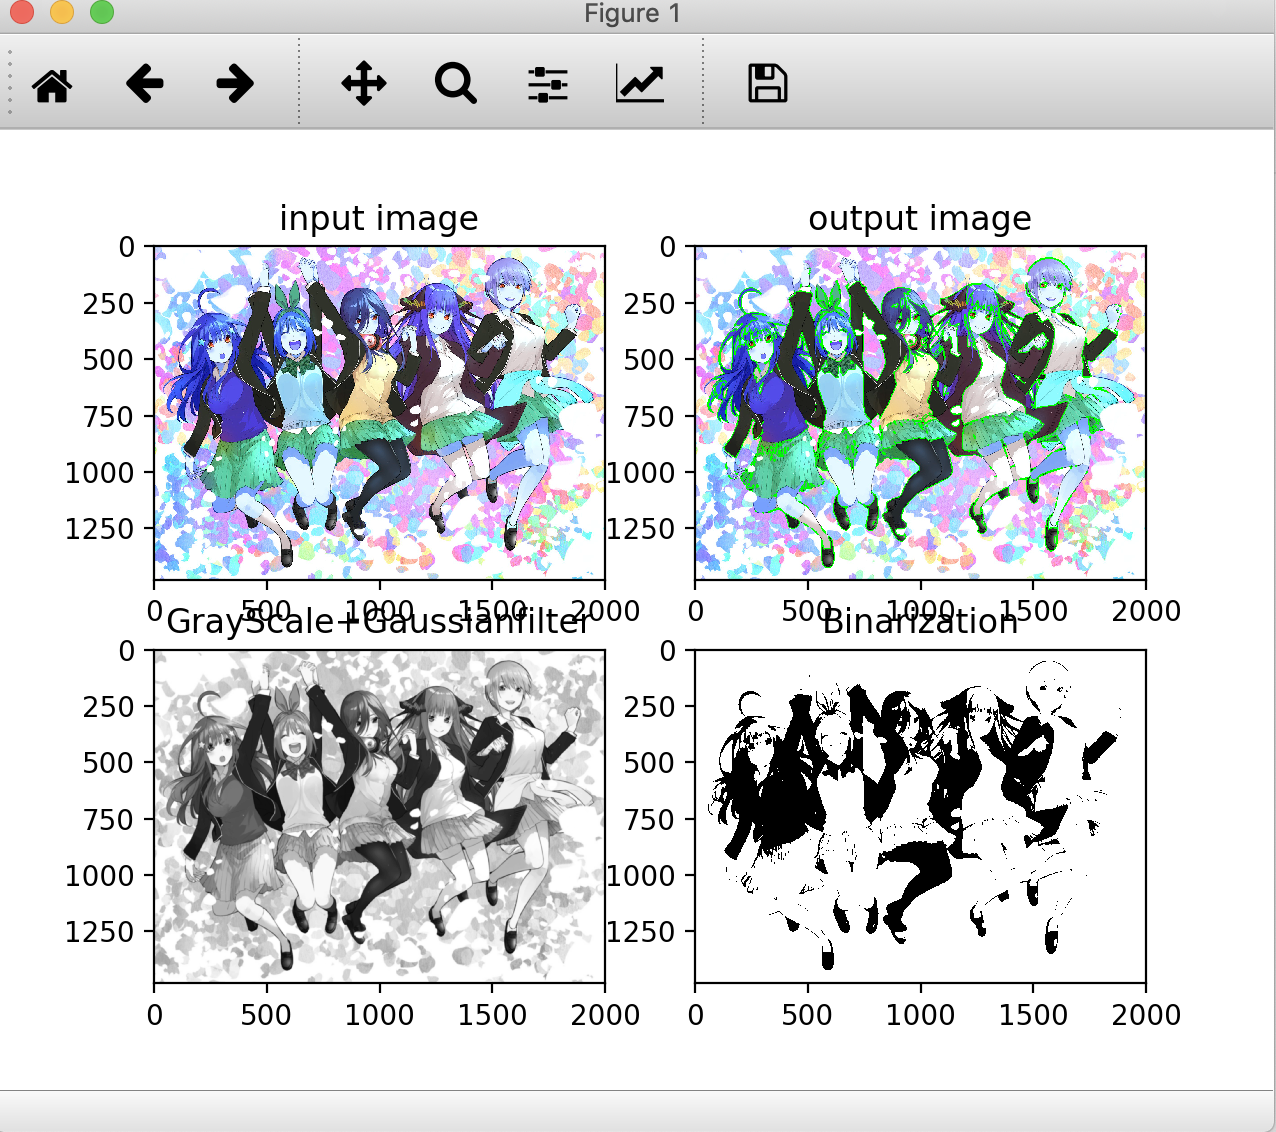
\includegraphics[clip, width=4.5cm]{./output2.png}
          \hspace{1.6cm} [2]結果画像その2
        \end{center}
        
      \end{minipage}
       \end{tabular}
    \caption{輪郭抽出}
    \label{fig:lena}
  \end{center}
\end{figure}

\begin{thebibliography}{99}
\bibitem{book1}
\bibitem{book2}
\end{thebibliography}
\end{document}


